%%%%%%%%%%%%%%%%%%%%%%%%%%%%%%%%%%%%%%%%%%%%%%%%%%%%%%%%%%%%%%%%%%%%%%%%%%%%%%%%
%2345678901234567890123456789012345678901234567890123456789012345678901234567890
%        1         2         3         4         5         6         7         8

\documentclass{ifacconf}  % Comment this line out if you need a4paper

\usepackage{natbib}        % required for bibliography
\usepackage{amsmath,empheq}
\usepackage{amsfonts}
\usepackage{amssymb}
\usepackage{txfonts}
\usepackage{acronym}

%todos
\usepackage[textsize=tiny,backgroundcolor=lightred,linecolor=red, bordercolor=red]{todonotes}
\usepackage{regexpatch}
\makeatletter
\xpatchcmd{\@todo}{\setkeys{todonotes}{#1}}{\setkeys{todonotes}{#1}}{}{}
\makeatother

\definecolor{lightred}{cmyk}{0,0.05,0,0} % pink
%%todos

\renewcommand{\vec}[1]{\boldsymbol{#1}}
%\newcommand*{\rom}[1]{\expandafter\@slowromancap\romannumeral #1@}
%\theoremstyle{definition}
\newtheorem{definition}{Definition}
%\documentclass[a4paper, 10pt, conference]{ieeeconf}      % Use this line for a4 paper
\newcounter{mytempeqncnt}
\usepackage{tikz}
%\IEEEoverridecommandlockouts                              % This command is only needed if 
                                                          % you want to use the \thanks command

%\overrideIEEEmargins                                      % Needed to meet printer requirements.

% See the \addtolength command later in the file to balance the column lengths
% on the last page of the document

% The following packages can be found on http:\\www.ctan.org
\usepackage{graphics} % for pdf, bitmapped graphics files
%\usepackage{epsfig} % for postscript graphics files
%\usepackage{mathptmx} % assumes new font selection scheme installed
%\usepackage{times} % assumes new font selection scheme installed
%\usepackage{amsmath} % assumes amsmath package installed
%\usepackage{amssymb}  % assumes amsmath package installed

\graphicspath{{figures/}}


%%%Acronyms

\acrodef{auv}[AUV]{autonomous underwater vehicle}
\acrodef{lqr}[LQR]{linear-quadratic regulator}
\acrodef{are}[ARE]{Algebraic Riccati Equation}
\acrodef{qlf}[QLF]{quadratic Lyapunov function}
\acrodef{cqlf}[CQLF]{common quadratic lyapunov function}
\acrodef{lmi}[LMIs]{linear matrix inequalities}
\acrodef{lti}[LTI]{linear time-invariant}
\acrodef{dof}[DoF]{degrees of freedom}
\acrodef{mimo}[MIMO]{multi-input multi-output}


\begin{document}
\begin{frontmatter}

\title{%\LARGE \bf
Modular Modeling and Trajectory Tracking LQ Regulator for Underwater Robots 
}

% \author{Yongyu Chen$^{1}$ and Stefan Sosnowski$^{1}$ and Sandra Hirche$^{1}$% <-this % stops a space
% % \thanks{*This work was not supported by any organization}% <-this % stops a space
% \thanks{$^1$ Chair of Information-oriented Control (ITR), Technical University of Munich (TUM),
%         {\tt\small yongyu.chen@tum.de, sosnowski@tum.de, hirche@tum.de}}%
% }


\author[First]{Yongyu Chen} 
\author[First]{Stefan Sosnowski} 
\author[First]{Sandra Hirche}

\address[First]{Chair of Information-oriented Control (ITR), Department of Electrical and Computer Engineering, Technical University of Munich (TUM), Germany (e-mail: \{yongyu.chen, sosnowski, hirche\}@tum.de).}
% \address[Second]{Chair of Information-oriented Control (ITR), Technical University of Munich (TUM),
%    Munich, Germany (e-mail: sosnowski@tum.de).}
% \address[Third]{Chair of Information-oriented Control (ITR), Technical University of Munich (TUM),
%    Munich, Germany (e-mail: hirche@tum.de).}


\begin{abstract}
In preparation for formulating the geometric design procedure of an \ac{auv} as an optimization problem, in this paper we introduce a new modular modeling approach. The focus is on the identification of the geometric parametrization and the parameter coupling both for the overall kinematic and kinetic design of the robot as well as the control allocation. In addition, we propose a method to formulate the robot dynamics as a linear \ac{mimo} switched system based on the task-determined trim trajectories and synthesize subsequently a switched \ac{lqr} controller, which can be checked for global stability. This enables a novel fully automatic task-dependent co-design of an \ac{auv} and its controller. Simulation results demonstrate that, in the unconstrained actuator case, the proposed model and control strategy can be successfully applied to perfectly track a set of predefined trim trajectories.
\end{abstract}




% In this work, we propose a modular modeling approach for reconfigurable underwater robots. Each component can be modeled as sample geometric shape determined by several geometric variables. The mass, moment of inertia and the hydrodynamic coefficients can be calculated from these geometric variables so that we can parametrize the robot dynamics with them. Besides, this paper addresses the problem of driving a underwater robot along predefined 3-D trim trajectories. This can be solved by formulating a trajectory-based  error system resulting in \acf{lti} error dynamics for each trim path. As a result, the nonlinear underwater robot dynamic system is transformed into a switched \ac{lti} system. For control strategy, we adopt switched a \ac{lqr} to drive the error states into zero. Simulation results where a underwater robot follows desired trim trajectories are presented to illustrate the performance of the proposed controller.


\begin{keyword}
autonomous vehicles, path planning, marine system, nonlinear control, global stability, linearization, mathematical models
\end{keyword}

\end{frontmatter}




% \maketitle
% \thispagestyle{empty}
% \pagestyle{empty}


%%%%%%%%%%%%%%%%%%%%%%%%%%%%%%%%%%%%%%%%%%%%%%%%%%%%%%%%%%%%%%%%%%%%%%%%%%%%%%%%


%!TEX root=../root.tex

%%%%%%%%%%%%%%%%%%%%%%%%%%%%%%%%%%%%%%%%%%%%%%%%%%%%%%%%%%%%%%%%%%%%%%%%%%%%%%%%
%2345678901234567890123456789012345678901234567890123456789012345678901234567890
%        1         2         3         4         5         6         7        
\section{INTRODUCTION}

% \todo{Reference to optimization goal, parametrization of dynamics with respect to set of optimization variables}
%When one module of the AUV is replaced by a new one whose data are already know, the modular modeling method is able to combine the new module and the remaining components to build a new dynamic model.

Typical design procedures for \acp{auv} involve standard models for submarine dynamics and an expert adapting these to the specific mission requirements. Often this is an iterative process, as many of the parameters are tightly coupled and immediately influence the dynamics and performance of the vehicle. Furthermore, due to the nonlinear, coupled nature of the vehicle dynamics, changes in the vehicle design parameters, such as a larger hull volume to accommodate more batteries, strongly affect the control design. We therefore aim to solve this challenge as a co-design process of a multi-criterion optimization of the vehicle kinematics and dynamics and a synthesis of a stable controller. The design requirements are specified through a given task, for example following a trajectory within a certain mission duration, which determines the necessary dynamics of the system and the power requirements. We opt for a task representation with trim trajectories as \emph{motion primitives} which can be combined to form arbitrarily complex paths.

An \ac{auv} is assembled from a collection of components (hull enclosure, batteries, fins, thrusters, CPU, inertial measurement unit, sensors, etc. ). In order to formulate the geometric design procedure of an \ac{auv} as an optimization algorithm, a modular model is required. It means that the shape and properties of each component of the underwater robot are parametrized by geometric variables, which in our case will be treated as optimization (i.e., decision) variables. The design requirements (e.g. being buoyancy neutral, low cost and maximum surge velocity) will be integrated in the objective function according to their relationship with these geometric decision variables. To design the underwater robot computationally is equivalent to solving the optimization problems and obtaining the feasible optimal solution. Modular geometry parametrized \ac{auv} models have been proposed before, see~\cite{c14} for \emph{A Simplified Dynamics Model for Autonomous Underwater Vehicles}, or~\cite{c15} and~\cite{c16} for \emph{Modular Modeling of Autonomous Underwater Vehicle}. The difference in our approach is that we parametrize the model with an emphasis on the coupling among all geometric decision variables and exposing them directly in the dynamic model formulation, enabling the optimization of the latter.

A computational way to design non-standard multicopters with optimization algorithms for a group of design goals was proposed by~\cite{c1}. Their algorithm iteratively optimizes the geometric (e.g., size, position and orientation) and the controller parameters of the constituent components (propellers, motors and carbon fiber-rods) under different metrics for specific applications. This novel approach enables the user to explore the geometric configuration space and discover robot structure significantly differing from the standard one. This robot geometry would be difficult to be modeled even by a experienced designer. Underwater robots are similar to multicopters in terms of the robot dynamics, both of which are rigid body with 6 \ac{dof} influenced by fluid dynamic effects. However, negligible aerodynamic effects become non-negligible in their hydrodynamic equivalents, making the models for the optimization more complex and requiring sophisticated control strategies. Therefore, we adopt a comparable approach to construct a customizable \ac{auv}. 



%The customizable robot structure implies the robot dynamics is determined by the number and the type of the constituent components and their geometric parameters. A more general and simpler dynamics modeling for reconfigurable underwater robot prototype is desired, which facilitates its design and dynamics analysis. 

%In~\cite{c2}, the components are modeled as simple geometric shapes with a few parameters. The hull is modeled as hollow cylinder with two solid spheres and the fins are assumed to be plate. In addition, the components including batteries and water bodies within the thruster housings which are not considered in~\cite{c1} are modeled as solid cylinders. The estimation methods of added mass coefficients and hydrodynamic coefficients for each components with simple geometric shapes are derived in detail in~\cite{c2}. 

% For trajectory-tracking control problem, the goal is to drive the position and velocity of the robot to track desired time-dependent position and velocity reference signals. We choose trim trajectory since robot's motion is stable along them. More precisely, the roll and pitch angles,
%The underwater water is a 6-DoF rigid body equivalent to the aerial robots. 
% By using the trim path for AUV, we obtain the equilibrium point for the nonlinear coupled robot dynamics. 
% \todo{Automatic co-design of controller and system for optimized geometry}

% \todo{How do these problems connect? We need to paint the whole picture and show why we combine the modeling with a trajectory representation and an automated control design}

To assess the current robot geometry, we use criteria for linear systems such as the condition number of the controllability matrix to judge different configurations of position and orientation of individual actuators . This requires a linearization of the naturally nonlinear and strongly coupled underwater robot dynamics and finding an appropriate equilibrium point is of significance. The concept of trim trajectories is suitable in this case as it corresponds to stable, steady-state, motions of the robot. More precisely, the roll and pitch angles, the dynamics states (linear and angular velocities) and the hydrodynamics terms depending on the velocities are constant. Trim trajectories used for path planning of aerial robots are described by~\cite{c2} and~\cite{c3}. Adopting the Frenet-Serret frame as the desired body frame for the motion, we can further derive the desired Euler angles and the Jacobian matrix. The equilibrium velocities values along trim paths can be computed from the position, Euler angles and the Jacobian matrix so that we can obtain the explicit values of the equilibrium points for the trim trajectory. In conclusion, the equilibrium points contain the full information of the trim trajectory specification.

Using trim trajectories as motion primitives, a complex trajectory could be constructed from a set of trim trajectories based on the mission requirements. For our trajectory-tracking approach, we follow the methodology reported in~\cite{c4}, \cite{c5} and \cite{c6} by defining the error states between the real robot states and the desired ones specified by the trim trajectories. The nonlinear error system can be linearized along the equilibrium point for a specific trim path, which results in a \ac{mimo} \ac{lti} system. In this way, the trim trajectory specifications are brought into the linearized error dynamics. Thus, we can utilize an \acf{lqr} to drive the generalized tracking error to zero. Suppose the combined trajectory consists of a set of $m$ trim trajectories, it is reasonable to formulate the nonlinear robot dynamics as a linear \ac{mimo} switched system with $m$ components and synthesize subsequently a switched \ac{lqr} controller to realize the path following. A constructive method to ensure the stability of the whole system under arbitrary switching is to find a \ac{cqlf} (\cite{c7}). The state and input weighting matrices can not be arbitrary selected. Their values must be chosen so that a \ac{cqlf} exists. If we utilize the controllability criteria of these $m$ linearized systems in the optimization algorithms, the robot geometry would also be determined by the predefined trajectory parameters.

%\todo{redundant}
%The main contribution of this work is to establish a generalized modular modeling approach for %underwater robot prototype. Its components are modeled as simple geometric shapes characterized with %several geometric parameters. We  can build the robot dynamics rapidly, when the geometric data are %offered. Besides, the trajectory error dynamics for a given set of trim paths is formulated as %switched system in this work. For which we adopt switched \ac{lqr} controller to control the robot's %motion. The proposed controller is then tested numerically by tracking a group of trim trajectory in %order to access its performance. 

This paper is organized as follows: Section II introduces the modular modeling approach of underwater robot dynamics and identifies the geometric decision variables. In Section III we elaborate how to find the equilibrium points for nonlinear underwater robot dynamics using trim trajectories. The formulation of the trajectory-based error space is discussed and the method for checking the existence of a \ac{cqlf} is presented. Simulation results illustrating the performance of the proposed control strategy are shown in Section V and Section VI presents the conclusion and future work.


%!TEX root=../root.tex

%%%%%%%%%%%%%%%%%%%%%%%%%%%%%%%%%%%%%%%%%%%%%%%%%%%%%%%%%%%%%%%%%%%%%%%%%%%%%%%%
%2345678901234567890123456789012345678901234567890123456789012345678901234567890
%        1         2         3         4         5         6         7        
\section{MODULAR MODELING}
The main components determining the shape and the dynamics of an \acp{auv} are the hull enclosing electronic internals and the actuators. The actuators can be further divided into thrusters and control fins. For the sake of simplicity and the computability of the overall model in the optimization process, we make the following assumptions:  (i) the hydrodynamic effects on the overall system are dominated by the effects on the hull and fins, those of the thrusters are negligible; (ii) the moment of inertia of the system is assumed to be merely determined by the hull components, fins and thrusters are neglected. 

\subsection{Modeling of Hull Components}
A world inertial frame $\left\{ i \right\}=(x_{i}~y_{i}~z_{i})$ describes the environment of the underwater robot which is fixed in space. The body-fixed reference frame $\left\{ b \right\}=(x_{b}~y_{b}~z_{b})$ for the whole robot is an accelerated coordinate frame fixed to the robot. The origin $o_{b}$ is usually chosen to coincide with the geometric center of the hull which will be referred to as $CO$. The longitudinal axis $x_{b}$ is directed from aft to fore, the transversal axis $y_{b}$ is directed to starboard and the normal axis $z_{b}$ orientates from top to bottom, see Fig.~\ref{FIG:HullThrusterGeometry}.

\begin{figure}[htb]
      \centering
      %\framebox{\parbox{3in}{We suggest that you use a text box to insert a graphic (which is ideally a 300 dpi TIFF or EPS file, with all fonts embedded) because, in an document, this method is somewhat more stable than directly inserting a picture.
%}}
      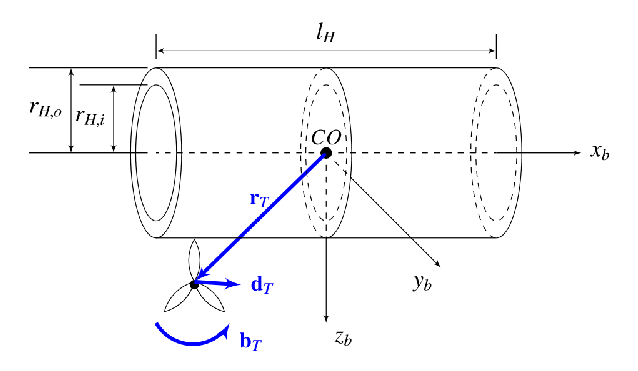
\includegraphics[scale=0.5]{HullThrusterGeometry.eps}
      \caption{Hull and thruster geometry}
      \label{FIG:HullThrusterGeometry}
\end{figure}
The main body typically embeds the navigation- , the sensory-  and the power supply-system. The shell is modeled as a hollow cylinder. We use three parameters to describe the dimensions: the inner radius $r_{H,i}$, the outer radius $r_{H,o}$ and the hull length $l_{H}$. Its mass $m_{H}$ is then calculated as $m_{H}=\rho_{H}\pi(r_{H,o}^{2}-r_{H,i}^{2})l_{H}$, with $\rho_{H}$ being the density of the hull material, and the moment of inertia with respect to its center of gravity can be calculated as follows:
\begin{align*}
I_{H}=diag([I_{xx,H}, I_{yy,H}, I_{zz,H}])
\end{align*}
where $I_{xx,H}=1/2m_{H}(r_{H,0}^{2}+r_{H,i}^{2})$ and $I_{yy,H}=I_{zz,H}=1/4m_{H}(r_{H,o}^{2}+r_{H,i}^{2}+l_{H}^{2}/3)$, due to its rotational symmetry along the $x_b$-axis and the symmetry with respect to the $z_{b}y_{b}-$plane. In the following, we use $r_{H}$ to represent $r_{H,o}$. Within the hull, we model the battery as a solid cylinder with length $l_{H}$ and radius $r_{H}$, the mass $m_{bat}=\rho \pi r_{bat}^{2}l_{bat}$ and the moment of inertia $I_{bat}$ with respect to the battery center of gravity is: 
\begin{align*}
I_{bat}=diag([I_{xx,bat}, I_{yy,bat}, I_{zz,bat}])
\end{align*}
where $I_{xx,bat}=I_{yy,bat}=1/12m_{bat}(3r_{bat}^{2}+l_{bat}^{2})$ and $I_{zz,bat}=1/2m_{bat}r_{bat}^{2}$.
%\begin{figure}[thpb]
     % \centering
      %\framebox{\parbox{3in}{We suggest that you use a text box to insert a graphic (which is ideally a 300 dpi TIFF or EPS file, with all fonts embedded) because, in an document, this method is somewhat more stable than directly inserting a picture.
%}}
     % 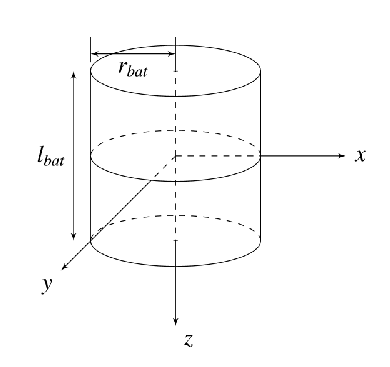
\includegraphics[scale=0.75]{BatModeling.eps}
     % \caption{Modeling of battery as solid cylinder}
     % \label{BatModel}
%\end{figure}
For all other electronic devices, we assume they have a constant mass $m_{d}$, volume $V_{d}$ and moment of inertia $I_{d}$ with respect to the robot body axes $\lbrace b \rbrace$.
For different underwater robot prototypes, the main customizable decision variables for the hull are its length $l_{H}$ and radius $r_{H}$ to enclose all internal devices and influence buoyancy. Therefore, we choose them as the decision variables of hull geometry and obtain the following definition:
\begin{definition}
The geometric decision parameters for the hull $\mathfrak{d}_{H}$ are defined as $\mathfrak{d}_{H}=\lbrace~l_{H}, r_{H}~|~l_{H}\in \mathbb{R}^{+}, r_{H} \in \mathbb{R}^{+}~\rbrace$, where $l_{H}$ denotes the length of the hull cylinder and $r_{H}$ is the radius of the hull cylinder.
\end{definition}
\subsection{Modeling of Thrusters}
As shown in Fig.~\ref{FIG:HullThrusterGeometry}, each thruster is parameterized by the motor orientation $\vec{d}_{T}$ (unit vector), the motor position $\vec{r}_{T}$ in the body frame $\lbrace b \rbrace$ and the motor spin direction $b_{T}\in \lbrace -1,1 \rbrace$, where -1 means counterclockwise and 1 represents clockwise. We use $u_{T}$ and $m_{T,r}$ to denote the magnitude of the thrust force and torque generated by the propeller rotation, respectively.
%\begin{figure}[thpb]
%      \centering
%      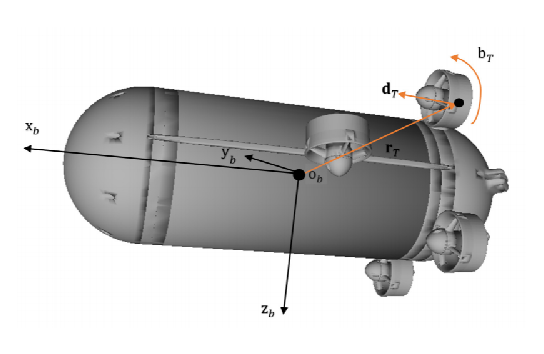
\includegraphics[scale=0.75]{thrusterlocation.eps}
%      \caption{Definition of thruster geometry}
%      \label{FIG:ThrusterLocation}
%\end{figure}
A simple one-state model for the propeller is proposed by~(\cite{c8}). If the propeller rotates in a steady state, the torque $m_{T,r}$ due to the rotation of a propeller is proportional to the thrust force. Thus, we can represent their relationship as $ m_{T,r}=\lambda_{T}u_{T}$, where $\lambda_{T}$ is the torque-force ratio. Taking the thruster motor orientation and the spin direction into consideration, we can obtain the rotation torque vector in $\lbrace b \rbrace$ as $\vec{m}_{T,r}=b_{T}\lambda_{T}u_{T}\vec{d}_{T}$. In addition, the thrust force will produce the thrust torque $\vec{m}_{T,t}$ relative to the center of gravity $CG$ of the complete robot. $CG$ is assumed to be located at the origin $CO$ of the body frame $\lbrace b \rbrace$. Then, the thrust torque can be calculated as $\vec{m}_{T,t}=\vec{r}_{T} \times u_{T}\vec{d}_{T}$, where $\vec{r}_{T} = (x_{T}~y_{T}~z_{T})^{T} \in \mathbb{R}^{3}$ is the position vector of the thruster in the body frame $\lbrace b \rbrace$. Combining the thrust torque and the rotation torque, we express the total torque produced by a thruster as $\vec{m}_{T}=\vec{m}_{T,r}+\vec{m}_{T,t}$. The force direction is determined by the thruster motor orientation $\vec{d}_{T}$ and the force vector $\vec{f}_{T}$ is written as $\vec{f}_{T}=u_{T}\vec{d}_{T} \in \mathbb{R}^{6}$. The generalized force vector $\vec{\tau}_{T}$ generated by a thruster is defined as $\vec{\tau}_{T}=(\vec{f}_{T}~\vec{m}_{T})^{T}\in \mathbb{R}^{6}$. If we treat the thrust force $u_{T}$ as the control input, we can define a unique vector $B_{T}$ mapping the thrust $u_{T}$ to the generalized force $\vec{\tau}_{T}$ as 
\begin{equation}
B_{T}=\begin{bmatrix}
\vec{d}_{T} \\
b_{T}\lambda_{T}\vec{d}_{T}+\vec{r}_{T} \times \vec{d}_{T}
\end{bmatrix} \in \mathbb{R}^{6}.
\end{equation}  
The generalized force produced by thrust force can thus be calculated as $\vec{\tau}=B_{T}u_{T}$. For the thrusters, we choose the geometric decision variables as follows:
\begin{definition}
The geometric parameter set for the thrusters $\mathfrak{d}_{P}$ is defined as $\mathfrak{d}_{P}=\lbrace~b_{T}, \vec{d}_{T}, \vec{r}_{T}~|~b_{T}\in \lbrace -1, 1 \rbrace, \vec{d}_{T} \in \mathbb{R}^{3}, \vec{r}_{T} \in \mathbb{R}^{3}~\rbrace$, where $b_{T}$ denotes the motor spin direction, $\vec{d}_{T}$ is the motor orientation and $\vec{r}_{T}$ represents the motor position.
\end{definition}
\subsection{Modeling of Control Fins}
The fins are approximated as rectangle with length $a_{F}$, width $b_{F}$ and negligible thickness. We assume the side edge $b_{F}$ is directly attached to the hull surface. The fins have a controllable \ac{dof} around an axis parallel to $a_{F}$ in the midsection of $b_{F}$. We represent the position and the orientation of the fins in the hull cylindrical coordinate system as illustrated in Fig.~\ref{FIG:FinGeo}, where $x_{F}$ is defined as the $x_b$-coordinate of the fin geometric center in robot body frame $\lbrace b \rbrace$. Then we rotate the $x_{b}z_{b}$-plane in the counterclockwise direction around $x_b$ by angle $\gamma_{F}$ until the fin geometric center is located in this plane. 
\begin{figure}[thpb]
\centering
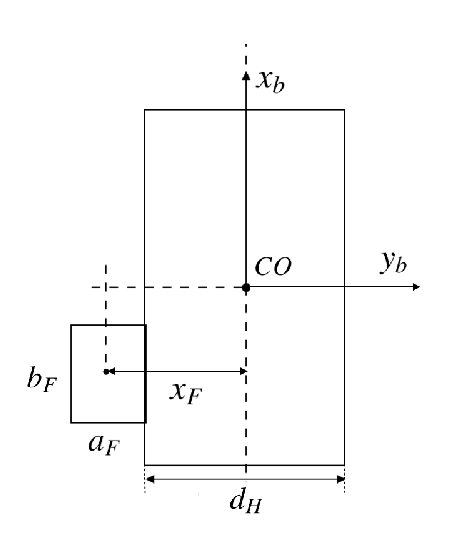
\includegraphics[width=1.25in]{finlocation1.eps}
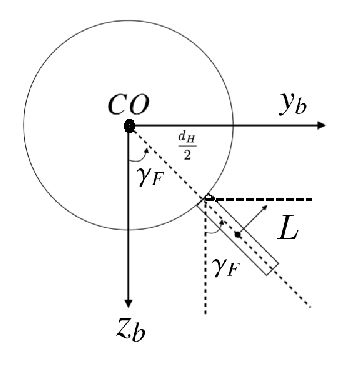
\includegraphics[width=1.25in]{finlocation2.eps}
\caption{Definition of fin geometry}
\label{FIG:FinGeo}
\end{figure}
As a result, the fin geometric center $\vec{r}_{F}$ in the robot body frame $\lbrace b \rbrace$ can be written as
\begin{equation}
\vec{r}_{F}=
\begin{bmatrix}
x_{F}\\0.5(d_{H}+a_{F})\sin(\gamma_{F})\\0.5(d_{H}+a_{F})\cos(\gamma_{F})
\end{bmatrix} \in \mathbb{R}^{3}.
\end{equation}
The unit vectors $\vec{e}_{1}=(0~0~1)^{T}$, $\vec{e}_{2}=(0~1~0)^{T}$ and $\vec{e}_{3}=(1~0~0)^{T}$ are the standard orthonormal basis of the robot body frame. 
We assume the fin velocity $\vec{v}_{fin}$ is equal to the robot velocity $\vec{v}$. For each fin, the lift $\vec{L}$ and drag $\vec{D}$ of fins can be calculated as
\begin{equation}
\vec{L}=0.5 \rho a_{F}b_{F}C_{L}(\alpha)||\vec{v}||^{2}
\begin{bmatrix}
0\\ \cos(\gamma_{F}) \\ -\sin(\gamma_{F})
\end{bmatrix} \in \mathbb{R}^{3},
\end{equation} and 
\begin{equation}
\vec{D} = 0.5 \rho a_{F}b_{F}C_{L}(\alpha)||\vec{v}||^{2}\vec{e}_{1} \in \mathbb{R}^{3},
\end{equation}
where $a_{F}$ and $b_{F}$ are the length and the width of the fin, respectively. $C_{L}$ is the lift coefficient and $C_{D}$ represents the drag coefficient, both of which are dependent on the angle of attack $\alpha$. Assuming the robot mainly moves forward, the surge velocity $u$ is dominant with respect to the sway $v$ and heave velocity $w$. Consequently, we can approximate $||\vec{v}||$ with $u$. Suppose the robot has $n_{f}$ fins, then the resultant force vector produced by all fins can be calculated as
\begin{equation}
\vec{f}_{F}(\alpha_{i})=
\begin{bmatrix}
\sum _{ i=1 }^{ n_{f} }{ \vec{L}_{ i }(\alpha _{ i })^{ T }\vec{e}_{ 1 }+ } \sum _{ i=1 }^{ n_{f} }{ \vec{D}_{ i }(\alpha _{ i })^{ T }\vec{e}_{ 1 } }  \\ \sum _{ i=1 }^{ n_{f} }{\vec{L}_{ i }(\alpha _{ i })^{ T }\vec{e}_{ 2 }+ } \sum _{ i=1 }^{ n_{f} }{ \vec{D}_{ i }(\alpha _{ i })^{ T }\vec{e}_{ 2 } }  \\ \sum _{ i=1 }^{ n_{f} }{ \vec{L}_{ i }(\alpha _{ i })^{ T }\vec{e}_{ 3 }+ } \sum _{ i=1 }^{n_{f} }{ \vec{D}_{ i }(\alpha _{ i })^{ T }\vec{e}_{ 3 } } 
\end{bmatrix} \in \mathbb{R}^{3}.
\end{equation} 
The resultant torque vector is calculated as 
\begin{equation}
\vec{\tau} _{F}(\alpha_{i} )=\sum _{ i=1 }^{n_{f}}{ \vec{r}_{F,i} \times \vec{L}_{i}(\alpha_{i}) } +\sum _{ i=1 }^{n_{f}}{ \vec{r}_{F,i} \times \vec{D}_{i}(\alpha_{i})}
\end{equation}
We regard the lift force as the input force and the drag as a disturbance. For small angles of attack $\alpha$ (about $15^\circ-20^\circ$), it is reasonable to approximate the lift and drag coefficient as $C_{L}(\alpha)=c_{L}\alpha$ and $C_{D}(\alpha)=c_{D}\alpha^{2}$, where $c_{L}$ and $c_{D}$ are fin-specific parameters measured from experiments, respectively. Furthermore, the angle of attack $\alpha$ can be approximated by the mechanical angle of rotation $\delta_{F}$ in the \ac{dof} of the fins. We treat $\delta_{F}$ as the control input for the fin actuators and define a mapping vector for each fin:  
\begin{equation}
B_{F}=\begin{bmatrix}
0\\0.5\rho c_{L}a_{F}b_{F} u^{2}\cos(\gamma_{F})\\
0.5\rho c_{L}a_{F}b_{F} u^{2}\sin(\gamma_{F})\\
-0.25\rho c_{L}a_{F}b_{F} u^{2}\sin(d_{H}+a_{F}) \\
0.5\rho c_{L}a_{F}b_{F} u^{2}x_{F}\sin(\gamma_{F})\\
0.5\rho c_{L}a_{F}b_{F} u^{2}x_{F}\cos(\gamma_{F})
\end{bmatrix} \in \mathbb{R}^{6}
\end{equation}
The fin mapping vector $B_{F}$ depends not only on the geometric parameters but also on the state of the rigid body due the existence of the surge velocity term, while the thruster mapping vector is only geometry-determined. The generalized force generated by the fins can be written as: $\vec{\tau}_{F}=(\vec{f}_{F}~\vec{m}_{F})^{T}=B_{F}\delta_{F}\in \mathbb{R}^{6}$. We select $x_{F}$ and $\gamma_{F}$ as decision variables for the fins:
\begin{definition}
The geometric parameter set for the fins $\mathfrak{d}_{F}$ is defined as $\mathfrak{d}_{F}=\lbrace~x_{F}, \gamma_{F}~|~x_{F}\in \mathbb{R}, \gamma_{F} \in (-\pi,\pi]~\rbrace$, where $x_{F}$ denotes the $x_b$-coordinate of the fin geometric center in the body frame $\lbrace b \rbrace$, $\gamma_{F}$ is the fin placement angle. 
\end{definition}
\subsection{Estimation of the Hydrodynamic Effects}
Hydrodynamic effects (added mass and hydrodynamic damping) are the distinct feature for underwater vehicles. Strictly speaking, each component (hull, thrusters and fins) contributes to the hydrodynamic forces and moments. They depend not only on the robot geometry but also on the inflow fluid velocity. Normally, the underwater robot dynamics are defined in the robot body frame $\lbrace b \rbrace$. However, the hydrodynamic effect of each module is calculated with respect to its own body frame. The calculated hydrodynamic effects need be transformed into the robot body frame $\lbrace b \rbrace$ according to the location of each module in $\lbrace b \rbrace$ to build the robot dynamics. This transformation results in nonlinearities and couplings between robot states and the actuator geometric variables. We assume that the added masses of thrusters and fins are negligible and only the added mass of the cylindrical hull is taken into consideration. The cylindrical hull has three planes of symmetry. The structure of the added mass inertia matrix $M_{A}$ and the added mass Coriolis matrix $C_{A}$ for a vehicle completely submerged in the water can be found in~\cite{c9}. The added mass coefficients can be calculated from the hull geometric parameters: $X_{\dot{u}}=-0.1m_{H}$, $Y_{\dot{v}}=Z_{\dot{w}}=-\pi \rho r_{H}^{2}l_{H}$, $K_{\dot{p}}=0$, $M_{\dot{q}}=N_{\dot{r}}=-1/12\pi \rho r_{H}^{2}l_{H}^{3}$. The damping matrix $D=diag([-X_{u|u|}|u|,-Y_{v|v|}|v|,-Z_{w|w|}|w|,-K_{p|p|}|p|,-M_{q|q|}|q|,-N_{r|r|}|r|])$,\\ the damping coefficients can be also calculated by the hull geometric parameters (see \cite{c10}). The damping coefficient in the $x_b$-direction due to the viscous force acting on the frontal area is given by $X_{u|u|}=-1/2\rho \pi C_{D}r_{H}^{2}$. The damping coefficients in the $y_b$- and $z_b$-axes due to the viscous effects on the side projected area of the hull are given as $Y_{|v|v}=Z_{|w|w}=-1/2\rho C_{D}2r_{H}l_{H}$. The hull has no contribution to the roll moment, hence $K_{p|p|}=0$. The pitch and yaw damping coefficients are equal due to the hull symmetry and given as $M_{q|q|}=N_{r|r|}=-1/12\rho C_{D}r_{H}l_{H}^{4}$ (see \cite{c11}). In this way, we establish the relationship between the explicit values of hydrodynamic terms and the geometric decision variables. 

\subsection{Dynamic Model}
%The moment of inertia of each individual module making up the robot is calculated with respect to the module's own body frame, while the hull frame is usually chosen as the reference body frame for the whole robot. This requires the individual moment of inertia to be transformed to the body frame $\lbrace b \rbrace$. 
%For each submodule whose center of gravity $CG_{s}$ is located in $\vec{r}_{G,s}=(x_{G,s}~y_{G,s}~z_{G,s})^{T}$  and the inertia matrix equals $diag([I_{xx,s}, I_{yy,s}, I_{zz,s}])$ in its own body frame, we can compute their moment of inertia in $\lbrace b \rbrace$ as follows: $I_{xx,s}^{b}=I_{xx,s}+m_{s}(y_{s}^{2}+z_{s}^{2})$, $I_{yy,s}^{b}=I_{yy,s}+m_{s}(z_{s}^{2}+x_{s}^{2})$, $I_{zz,s}^{b}=I_{zz,s}+m_{s}(x_{s}^{2}+y_{s}^{2})$, where $I_{xx,s}^{b}$, $I_{yy,s}^{b}$ and $I_{zz,s}^{b}$ are moments of inertia with respect to the body axes $\lbrace b \rbrace$ of the component $s$.
%Suppose we have totally $N$ components, then the resultant center of mass $\vec{r}_{G}$ for the whole robot is 
%\begin{equation}
%\vec{r}_{G}=\frac{\sum_{s=1}^{N}m_{s}\vec{r}_{G,s}}{\sum_{s=1}^{N}m_{s}}.
%\end{equation}
%$\vec{r}_{G}$ is determined by $\mathfrak{d}_{P}$, $\mathfrak{d}_{H}$ and $\mathfrak{d}_{F}$. 
The state variables of underwater robots can be divided into two groups, i.e., kinematic and dynamic states. Dynamic states consist of three linear and three angular velocities represented in the robot body frame $\lbrace b \rbrace$: $\vec{x}_{dyn}=(\vec{v}~\vec{\omega})^{T}=(u~v~w~p~q~r)^{T} \in \mathbb{R}^{6}$. Kinematic states consist of the position and orientation of the underwater robot in the inertial world frame $\lbrace i \rbrace$: $\vec{x}_{kin}=(\vec{p}~\vec{\eta})^{T}
=(x~y~z~\phi~\theta~\psi)^{T} \in \mathbb{R}^{6}$. The complete states are defined as $\vec{x}=(\vec{x}_{dyn}~\vec{x}_{kin})^{T} \in \mathbb{R}^{12}$. 
The standard underwater robot dynamic equation is given by
\begin{equation}
M\begin{bmatrix}
\dot{\vec{v}} \\
\dot{\vec{w}}
\end{bmatrix}+
C(\vec{v},\vec{w})\begin{bmatrix}
\vec{v} \\
\vec{w}
\end{bmatrix}+
D(\vec{v},\vec{w})\begin{bmatrix}
\vec{v}\\
\vec{w}
\end{bmatrix}+\vec{g}(\vec{\eta})=\vec{\tau}. \label{EQ:RobotDynamics}
\end{equation}
Based on the modular modeling, each term in (\ref{EQ:RobotDynamics}) can be uniquely computed from the predefined groups of geometric decision variables. 
\begin{equation}
M:=M_{RB}(\mathfrak{d}_{H}, \mathfrak{d}_{P}, \mathfrak{d}_{F})+M_{A}(x_{dyn}, \mathfrak{d}_{H})  
\end{equation} 
is the generalized mass matrix of the underwater robot with $M_{RB}$ and $M_{A}$ representing the rigid body mass matrix and the added mass matrix, respectively. Furthermore, 
\begin{equation}
   C(\vec{v},\vec{w}):=C_{RB}(\vec{x}_{dyn}, \mathfrak{d}_{H}, \mathfrak{d}_{P}, \mathfrak{d}_{F})+C_{A}(\vec{x}_{dyn}, \mathfrak{d}_{H})
 \end{equation} is the Coriolis-centripetal matrix (including added mass effects), $D(\vec{x}_{dyn}, \mathfrak{d}_{H})$ is the damping matrix and $\vec{g}(\vec{\eta})$ is the vector of gravitational/buoyancy forces and moments, which can be written in the geometry-dependent form as $\vec{g}({\vec{x}_{kin}, \mathfrak{d}_{H}, \mathfrak{d}_{P}, \mathfrak{d}_{F}})$. $\vec{\tau}$ is the generalized force vector generated by thrusters and control surfaces (fins). We use $\vec{u}_{T}$ and $\vec{u}_{F}$ to denote the control inputs generated by thrusters and fins, respectively. Suppose the robot has $n_{t}$ thrusters and $n_{f}$ fins, then the thruster input vector can be written as $\vec{u}_{T}=(u_{T,1}, \cdots, u_{T,n_{t}})^{T} \in \mathbb{R}^{n_{t} \times 1}$ and the fin input vector is defined as $\vec{u}_{F}=(\delta_{F,1}, \cdots, \delta_{F,n_{f}})^{T} \in \mathbb{R}^{n_{f} \times 1}$. The complete input vector for the robot system is defined as $\vec{u}=(\vec{u}_{T}~\vec{u}_{F})^{T} \in \mathbb{R}^{(n_{t}+n_{f}) \times 1}$. For each actuator, there is a corresponding input mapping vector and we can formulate the thruster input matrix as $B_{a,T}=(B_{T,1} \cdots B_{T,n_{t}})\in \mathbb{R}^{6\times n_{t}}$. The fin input matrix is defined as $B_{a,F}=(B_{F,1} \cdots B_{F,n_{t}})\in \mathbb{R}^{6\times n_{f}}$. Stacking them together, we get the input mapping matrix $B_{a}=(B_{a,T}~B_{a,F})^{T} \in \mathbb{R}^{6 \times (n_{t}+n_{f})}$. Thus, we obtain the relationship $\vec{\tau}=B_{a}\vec{u}$. Given a robot prototype with known geometric data of all components, we can directly construct the dynamic equation for analysis. 


%!TEX root=../root.tex

%%%%%%%%%%%%%%%%%%%%%%%%%%%%%%%%%%%%%%%%%%%%%%%%%%%%%%%%%%%%%%%%%%%%%%%%%%%%%%%%
%2345678901234567890123456789012345678901234567890123456789012345678901234567890
%        1         2         3         4         5         6         7        
\section{TRAJECTORY-DEPENDENT ERROR SYSTEM}
In this section, we introduce the transformation of the underwater dynamic model into an error system when the robot tracks a trim trajectory. Moreover, the linearization of the error dynamics is discussed.
 
\subsection{Frenet-Serret Frame}
When the robot moves along a smooth curve $\vec{r}(t)=(x(t)~y(t)~z(t))^{T}$ in the three-dimensional Euclidean space $\mathbb{R}^{3}$, its motion can be characterized by three unit vectors: $T^{i}(t)$, $N^{i}(t)$ and $B^{i}(t)$. $T^{i}(t)$ is a unit vector tangent to the curve denoting the motion direction, which can be calculated as the changing rate of the curve vector with respect to its arclength $s$:
\begin{equation}
T^{i}(t)=\dfrac{d\vec{r}}{ds}=\frac{\vec{r}^{'}(t)}{||\vec{r}^{'}(t)||}.
\end{equation}
The normal vector $N^{i}(t)$ is defined as the derivative of $T^{i}$  with respect to the arclength $s$ of the curve, divided by its length:
\begin{equation}
N^{i}(t)=\dfrac{\dfrac{dT^{i}(t)}{ds}}{\left|\left|\dfrac{dT^{i}(t)}{ds}\right|\right|}=\dfrac{(T^{i})^{'}(t)}{||(T^{i})^{'}(t)||}=\dfrac{\vec{r}^{'}(t)\times (\vec{r}^{''}(t)\times \vec{r}^{'}(t))}{||\vec{r}^{'}(t)||~||\vec{r}^{''}(t)\times \vec{r}^{'}(t)||}.
\end{equation}
The binormal vector $B^{i}_{T}$ is the cross product of the normal vector $N^{i}(t)$ and the tangent vector $T^{i}(t)$ and is calculated as 
\begin{equation}
B^{i}(t)=T^{i}(t)\times N^{i}(t)=\frac{\vec{r}^{''}(t)\times \vec{r}^{'}(t)}{||\vec{r}^{''}(t)\times \vec{r}^{'}(t)||}.
\end{equation}
\subsection{Trim Trajectory}
The concept of trim trajectories originates in the path planning for aircrafts. It corresponds to a curve $\vec{p}_{\mathcal{T}}=(x_{\mathcal{T}}~y_{\mathcal{T}}~z_{\mathcal{T}})^{T}
\in \mathbb{R}^{3}$ that the robot can follow in a steady-state equilibrium. A trim trajectory $\vec{p}_{\mathcal{T}}$ is parametrized by three parameters $\vec{p}_{\mathcal{T}}: (||\vec{v}_{\mathcal{T}}||~\dot{\phi}_{\mathcal{T}}~\gamma_{T})^{T}$, where $\vec{v}_{\mathcal{T}}$ is the trim speed. We choose the aforementioned Frenet-Serret frame as the desired body frame for the robot moving along the trim trajectory curve and denote it as $\lbrace \mathcal{T} \rbrace$. The desired orientation on basis of $\lbrace \mathcal{T} \rbrace$ for the trim trajectory is represented as $\vec{\eta}_{\mathcal{T}}=(\phi_{\mathcal{T}}~\theta_{\mathcal{T}}~\psi_{\mathcal{T}})^{T}$. For $\lbrace \mathcal{T} \rbrace$, the trim speed is equal to the desired surge velocity $u$. The angle $\gamma_{\mathcal{T}}$ is the flight path angle. The trim yaw angle is given by $\phi_{\mathcal{T}}(t)=\dot{\phi}_{\mathcal{T}}t+\phi_{0}$, where $\dot{\phi}_{\mathcal{T}}\in \mathbb{R}$ is the constant yaw rate and $\phi_{0}\in [0,2\pi)$ is the initial yaw angle. Along the trim trajectory, the roll and pitch angle remain unchanged, i.e., $\dot{\phi}_{\mathcal{T}}=0$ and $\dot{\theta}_{\mathcal{T}}=0$. 
\begin{figure}[thpb]
\centering
\includegraphics[width=2.5in]{trimtraj.eps}
\caption{Trim trajectory}
\label{FinGeo}
\end{figure} 
A trim trajectory segment corresponds to a helix with radius $||\vec{v}_{\mathcal{T}}||\dot{\psi}_{\mathcal{T}}^{-1}\cos(\gamma_{\mathcal{T}})$ and is represented as
\begin{align}
&\vec{p}_{\mathcal{T}}(t)= \nonumber
\\&||\vec{v}_{\mathcal{T}}||\dot{\psi}_{\mathcal{T}}^{-1}\cos(\gamma_{\mathcal{T}})
\begin{bmatrix}
\sin(\psi_{\mathcal{T}}(t)-\psi_{v})-\sin(\psi_{0}-\psi_{v}) \\
\cos(\psi_{\mathcal{T}}(t)-\psi_{v})+\cos(\psi_{0}-\psi_{v}) \\
-\dot{\psi}_{\mathcal{T}}\tan(\gamma_{\mathcal{T}})t
\end{bmatrix}+
\vec{p}_{0},\label{EQ:pT}
\end{align}
where $\vec{p}_{0}=(x_{0}~y_{0}~z_{0})^{T} \in \mathbb{R}^{3}$ is the initial trim position.
The transformation matrix from the Frenet-Serret frame $\lbrace \mathcal{T} \rbrace$ to the inertial world frame $\lbrace i \rbrace$ is defined as $
 \mathcal{R}_{\mathcal{T}}:=
 (T^{i}(t)~N^{i}(t)~B^{i}(t))$. The desired trim roll and pitch angle can be inferred from the Frenet-Serret frame setting as $\theta_{\mathcal{T}}=-\sin^{-1}(\vec{T}^{i}(t))$ and $
\phi_{\mathcal{T}}=-\sin^{-1}(\sec(\theta_{\mathcal{T}})\cdot \vec{N}^{i}(t))
$, respectively. Stacking the two dynamic-affecting angles together we define $\vec{\eta}_{p,\mathcal{T}}=(\phi_{\mathcal{T}}~\theta_{\mathcal{T}})^{T}$. With the value of $\phi_{\mathcal{T}}$ and $\theta_{\mathcal{T}}$, we can obtain the angular velocity transformation matrix $\mathcal{Q}_{\mathcal{T}}$. Thus, the desired velocities along the trim trajectory can be calculated as
\begin{equation}
\begin{bmatrix}
\vec{v}_{\mathcal{T}} \\
\vec{w}_{\mathcal{T}}
\end{bmatrix} =
\begin{bmatrix}
\mathcal{R}_{\mathcal{T}}^{-1} & 0\\
0 & \mathcal{Q}_{\mathcal{T}}^{-1} 
\end{bmatrix}
\begin{bmatrix}
\vec{p}_{\mathcal{T}} \\ \vec{\eta}_{\mathcal{T}}
\end{bmatrix}.
\end{equation}
All the variables affecting the underwater robot dynamics ($\vec{v}_{\mathcal{T}}$, $\vec{w}_{\mathcal{T}}$, $\vec{\eta}_{p,\mathcal{T}}$), see~(\ref{EQ:RobotDynamics}), stay constant. They correspond to the equilibrium point for motion along the trim trajectory. The equilibrium input corresponding to $\dot{\vec{v}}_{\mathcal{T}}=\vec{0}$ and $\dot{\vec{w}}_{\mathcal{T}}=\vec{0}$ can be calculated as
\begin{align}
\vec{\tau}_{d,\mathcal{T}}=&C_{RB}(\vec{x}_{dyn,\mathcal{T}},\vec{r}_{T},\mathfrak{d}_{H},\mathfrak{d}_{F})
\begin{bmatrix}
\vec{v}_{\mathcal{T}} \\ \vec{w}_{\mathcal{T}}
\end{bmatrix}
+ 
C_{A}(\vec{x}_{dyn,\mathcal{T}},\mathfrak{d}_{H})\vec{\upsilon}_{\mathcal{T}}+ \nonumber \\ & D(\vec{x}_{dyn,\mathcal{T}},\mathfrak{d}_{H})\vec{\upsilon}_{\mathcal{T}} 
+\vec{g}(\vec{x}_{kin,\mathcal{T}},\mathfrak{d}_{F},\vec{r}_{T},\mathfrak{d}_{H}).
\end{align}
The underwater dynamics can be linearized for explicit values of $\vec{v}_{\mathcal{T}}, \vec{w}_{\mathcal{T}}$, $\vec{\eta}_{p,\mathcal{T}}$ and $\vec{u}_{\mathcal{T}}$. 
The state space form of the underwater robotic system is given by
\begin{equation}
\frac{d}{dt}\begin{bmatrix}
\vec{x}_{dyn} \\
\vec{x}_{kin}
\end{bmatrix}=
\begin{bmatrix}
\vec{f}_{dyn}(\vec{x}_{dyn},\vec{x}_{kin}) \\
\vec{f}_{kin}(\vec{x}_{dyn},\vec{x}_{kin})
\end{bmatrix} +
\begin{bmatrix}
\vec{g}_{dyn}(\vec{x}_{dyn},\vec{u}) \\
\vec{0}
\end{bmatrix}.
\end{equation}
Equivalently, they can be written in the following form:
\begin{empheq}[left=\empheqlbrace]{align}
& \frac{d}{dt}\vec{v}=\vec{f}_{\vec{v}}(\vec{v},\vec{w})+\vec{f}_{\vec{v}}^{\vec{\eta}}(\vec{\eta}_{p})+\vec{g}_{\vec{v}}
(\vec{v},\vec{u}) \label{EQ:SS_v} \\
&\frac{d}{dt}\vec{w}=\vec{f}_{\vec{w}}(\vec{v},\vec{w})+
\vec{f}_{\vec{w}}^{\vec{\eta}}(\vec{\eta}_{p})+
\vec{g}_{\vec{w}}
(\vec{v},\vec{u}) \label{EQ:SS_w} \\
& \frac{d}{dt}\vec{p} =\mathcal{R}(\vec{\eta})\vec{v}  \\
&\frac{d}{dt}\vec{\eta}=\mathcal{Q}(\vec{\eta}_{p})\vec{\omega}.
\end{empheq}
where $\vec{\eta}_{p}=(\phi~\theta)^{T}$ denotes the partial kinematic states affecting the underwater robot dynamics appearing in the restoring term $\vec{g}(\vec{\eta})$, $\mathcal{R}$ is the linear velocity transformation matrix from $\lbrace b \rbrace$ to $\lbrace i \rbrace$ and $\mathcal{Q}$ is the transformation matrix  relating the body fixed angular velocity $\vec{w}$ to Euler angle rates. We now need to convert (\ref{EQ:RobotDynamics}) into the state space form, see (\ref{EQ:SS_v}) and (\ref{EQ:SS_w}).  

The first three rows of the matrix $B_{a}$ are denoted by $B_{a,f}\in \mathbb{R}^{3\times(n_{t}+n_{f})}$ and the last three rows of the matrix are represented by $B_{a,m}\in \mathbb{R}^{3\times(n_{t}+n_{f})}$. The generalized force generated by the actuators can be represented as $\vec{\tau}=B_{a}\vec{u}$. Separately written, $\vec{f}=\emph{\textbf{B}}_{a,f}\vec{u}$ and $\vec{m}=\emph{\textbf{B}}_{a,m}\vec{u}$, where $\vec{f}$ is the force vector along the $x_b$-, $y_b$- and $z_b$-axes of $\lbrace b \rbrace$ and $\vec{m}$ is the moment vector about  those axes. Hence, for our modeling approach, we get $\vec{g}_{\vec{v}}(\vec{v},\vec{u})=M^{-1}B_{a,f}\vec{u}$ and
$\vec{g}_{\vec{w}}(\vec{v},\vec{u})=M^{-1}B_{a,m}\vec{u}$. The rigid body Coriolis-centripetal matrix $C_{RB}(\vec{v},\vec{w})$ can be separated into $C_{RB,\vec{v}}$ and $C_{RB,\vec{w}}$ corresponding to the first and last three rows of the Coriolis matrix $C_{RB}$, respectively. Similarly, we assign the first three lines of the added mass Coriolis matrix $C_{A}$ to $C_{A,\vec{v}}(\vec{v},\vec{w})$ and the last three lines to $C_{A,\vec{w}}(\vec{v},\vec{w})$. 
%\begin{equation}
%\emph{\textbf{C}}_{A,\vec{w}}(\vec{v},\vec{w})=
%\begin{bmatrix}
%0&-Z_{\dot{w}}w&Y_{\dot{v}}v&0&-N_{\dot{r}}\dot{r}&M_{\dot{q}}q\\
%Z_{\dot{w}}w&0&-X_{\dot{u}}u&N_{\dot{r}}r&0&-K_{\dot{p}}p\\
%-Y_{\dot{v}}v&X_{\dot{u}}u&0&-M_{\dot{q}}q&K_{\dot{p}}p&0
%\end{bmatrix}
%\end{equation}
The restoring vector $\vec{g}(\vec{\eta})$ can also be separated in the same way into $\vec{g}_{\vec{v}}(\vec{\eta})\in \mathbb{R}^{3}$ that is the first three elements of $\vec{g}(\vec{\eta})$ and $\vec{g}_{\vec{w}}(\vec{\eta})\in \mathbb{R}^{3}$ corresponding to the last three elements. 
To sum up, we can obtain the following relationship between the terms in the underwater robot dynamics and the state-space terms:
\begin{align}
\vec{f}_{\vec{v}}(\vec{v},\vec{w})&=-M^{-1}(C_{RB,\vec{v}}+C_{A,\vec{v}}+D_{\vec{v}}), \label{EQ:fv}\\
\vec{f}_{\vec{w}}(\vec{v},\vec{w})&=-M^{-1}(C_{RB,\vec{w}}+C_{A,\vec{w}}+D_{\vec{w}}), \label{EQ:fw} \\
\vec{f}_{\vec{v}}^{\vec{\eta}}(\vec{\eta}_{p})&=-M^{-1}\vec{g}_{\vec{v}}(\vec{\eta}), \label{EQ:fveta}\\
\vec{f}_{\vec{w}}^{\vec{\eta}}(\vec{\eta}_{p})&=-M^{-1}\vec{g}_{\vec{w}}(\vec{\eta})\label{EQ:fweta}.
\end{align}
%\begin{figure*}[!t]
% ensure that we have normalsize text
%\normalsize
% Store the current equation number.
%\setcounter{mytempeqncnt}{\value{equation}}
% Set the equation number to one less than the one
% desired for the first equation here.
% The value here will have to changed if equations
% are added or removed prior to the place these
% equations are referenced in the main text.
%\setcounter{equation}{5}
%\begin{equation}
%\label{eqn_dbl_x}
%\emph{\textbf{C}}_{RB,\vec{v}}= \\
%\begin{bmatrix}
%0&0&0&m(y_{g}q+z_{g}r)&-m(x_{g}q-w)&-m(x_{g}r+v)\\
%0&0&0&-m(y_{g}p+w)&m(z_{g}r+x_{g}p)&-m(y_{g}r-u)\\
%0&0&0&-m(z_{g}p-v)&-m(z_{g}q+u)&m(x_{g}p+y_{g}q)\\
%\end{bmatrix} 
%\end{equation}
%\begin{gather}\label{EQ:CoriolisRigidBodyW}
%\emph{\textbf{C}}_{RB,\vec{\omega}}(\vec{v},\vec{\omega})=
%\left[
%\begin{matrix} -m(y_{g}+z_{g}r)&m(y_{g}p+w)&m(z_{g}p-v)\\
%m(x_{g}q-w)&-m(z_{g}r+x_{g}p)&m(z_{g}q+u)\\
%m(x_{g}r+v)&m(y_{g}r-u)&-m(x_{g}p+y_{g}q)
%\end{matrix}
%\right.
% \nonumber\\
%\qquad \qquad\left. \begin{matrix} 
%0 & -I_{yz}q-I_{xz}p+I_{z}r & I_{yz}r+I_{xy}p-I_{y}q \\
%I_{yz}q+I_{xz}p-I_{z}r &0& -I_{xz}r-I_{xy}q+I_{x}p \\
%-I_{yz}r-I_{xy}p+I_{y}q&I_{xz}r+I_{xy}q-I_{x}p &0  \end{matrix}
%\right]
%\end{gather}
%\begin{equation}
%\vec{g}_{\vec{v}}(\vec{\eta})=
%\begin{bmatrix}
%(W-B)\sin(\theta)\\
%-(W-B)\cos(\theta)\sin(\phi)\\
%-(W-B)\cos(\theta)\cos(\phi)
%\end{bmatrix}\label{EQ:RstV}
%\end{equation}
%\begin{equation}
%\vec{g}_{\vec{\omega}}(\vec{\eta})=
%\begin{bmatrix}
%-(y_{g}W-y_{b}B)\cos(\theta)\cos(\phi)+(z_{g}W-%z_{b}B)\cos(\theta)\sin(\phi)\\
%(z_{g}W-z_{b}B)\sin(\theta)+(x_{g}W-x_{b}B)\cos(\theta)\cos(\phi)\\
%-(x_{g}W-x_{b}B)\sin(\theta)\cos(\phi)-(y_{g}W-y_{b}B)\sin(\theta)
%\end{bmatrix}\label{EQ:RstW}
%\end{equation}
% Restore the current equation number.
%\setcounter{equation}{\value{mytempeqncnt}}
% IEEE uses as a separator
%\hrulefill
% The spacer can be tweaked to stop underfull vboxes.
%\vspace*{4pt}
%\end{figure*}
\subsection{Nonlinear Transformation and Error Dynamics}
Fig.~\ref{FIG:FrameRelationship} shows the relationship between the inertial world frame $\lbrace i \rbrace$, the robot body frame $\lbrace b \rbrace$ and the Frenet-Serret frame along the trim curve $\lbrace \mathcal{T} \rbrace$. In the ideal case, the robot body frame $\lbrace b \rbrace$ should coincide with the frame $\lbrace \mathcal{T} \rbrace$ for perfect tracking, but it is not necessarily the case in reality. Therefore, we use $\mathcal{R}_{E}$ to denote  the transformation matrix from $\lbrace b \rbrace$ to $\lbrace \mathcal{T} \rbrace$ for linear velocities and position and $\mathcal{Q}_{E}$ for angular velocities. Based on these definitions, we have the following relationship $\mathcal{R}_{E}=\mathcal{R}_{\mathcal{T}}^{-1}\mathcal{R}$ and $\mathcal{Q}_{E}=\mathcal{Q}_{\mathcal{T}}^{-1}\mathcal{Q}$. We adopt the following transformation for the state errors: $\vec{v}_{E}=\vec{v}-\vec{v}_{\mathcal{T}}$, $\vec{w}_{E}=\vec{w}-\vec{w}_{\mathcal{T}}$, $\vec{p}_{E}=\mathcal{R}^{-1}(\vec{p}-\vec{p}_{\mathcal{T}})$ and $\vec{\eta}_{E}=\mathcal{R}^{-1}(\vec{\eta}-\vec{\eta}_{\mathcal{T}})$, which can be interpreted as the errors 
between the desired trim states and the real robot states as measured by sensors in the robot body frame $\lbrace b \rbrace$. We define the error dynamics input as $\vec{u}_{E}=\vec{u}-\vec{u}_{\mathcal{T}}$, where $\vec{u}$ is the control input from the actuators and $\vec{u}_{\mathcal{T}}$ is the desired trim actuator input, which is calculated as $\vec{u}_{\mathcal{T}}=B_{a}^{-1}\vec{\tau}_{d,\mathcal{T}}$.
\begin{figure}[thpb]
\center
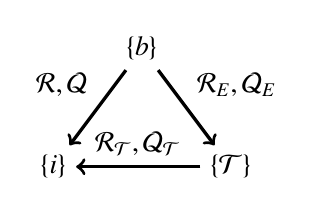
\begin{tikzpicture}[scale=0.75]
\node (A) at (0,0){$\lbrace i \rbrace$};
\node (B) at (1.5,2){$\lbrace b \rbrace$};
\node (C) at (3,0){$\lbrace \mathcal{T} \rbrace$};
\draw[->, very thick] (B) to
node[above left] {$\mathcal{R}, \mathcal{Q}$} (A);
\draw[->, very thick] (C) to
node[above] {$\mathcal{R}_{\mathcal{T}}, \mathcal{Q}_{\mathcal{T}}$} (A);
\draw[->, very thick] (B) to
node[above right] {$\mathcal{R}_{E}, \mathcal{Q}_{E}$} (C);
\end{tikzpicture}
\caption{Frame relationship}	
\label{FIG:FrameRelationship}
\end{figure}

\subsection{Linearization of Error System}
In the previous section, we have derived the equilibrium point for the motion of the \ac{auv} along a trim trajectory and defined the error system for tracking this trajectory. It is common to control a nonlinear system by linearizing it at an equilibrium point. Moreover, we can use properties of the linearized system as performance criteria for finding an optimal geometry, e.g., the controllability matrix. Thus, in this section, we perform the linearization of (\ref{EQ:fv}), (\ref{EQ:fw}), (\ref{EQ:fveta}) and (\ref{EQ:fweta}) at ($\vec{v}_{\mathcal{T}}$, $\vec{w}_{\mathcal{T}}$, $\vec{\eta}_{p,\mathcal{T}}$, $\vec{u}_{\mathcal{T}}$),

\begin{empheq}[left=\empheqlbrace]{align}
&\dfrac{d}{dt}\delta\vec{v}_{E}=A_{\vec{v}}^{\vec{v}}
\delta\vec{v}_{E}+A_{\vec{v}}^{\vec{\omega}}
\delta\vec{\omega}_{E}+A_{\vec{v}}^{\vec{\eta}}
\delta\vec{\vec{\eta}}_{E}+B_{\vec{v}}\delta\vec{u} \\
&\dfrac{d}{dt}\delta\vec{w}_{E}=A_{\vec{w}}^{\vec{v}}
\delta\vec{v}_{E}+A_{\vec{w}}^{\vec{w}}
\delta\vec{w}_{E}+A_{\vec{w}}^{\vec{\eta}}
\delta\vec{p}_{E}+B_{\vec{w}}\delta\vec{u} 
\end{empheq} 
where
\begin{empheq}[left=\empheqlbrace]{align}
&A_{\vec{v}}^{\vec{v}}=\dfrac{\partial}{\partial \vec{v}}[\vec{f}_{\vec{v}}(\vec{v},\vec{w})+\vec{g}_{\vec{v}}(\vec{v},\vec{w},\vec{u})]
 \\
&A_{\vec{v}}^{\vec{w}}=\dfrac{\partial}{\partial \vec{w}}[\vec{f}_{\vec{v}}(\vec{v},\vec{w})+\vec{g}_{\vec{v}}(\vec{v},\vec{w},\vec{u})]
\\
&A_{\vec{v}}^{\vec{\eta}}=\dfrac{\partial}{\partial \vec{\eta}}\vec{f}_{\vec{v}}^{\vec{\eta}}(\vec{\eta}_{p})\\
&B_{\vec{v}}=\dfrac{\partial}{\partial \vec{u}}
\vec{g}_{\vec{v}}(\vec{v},\vec{w},\vec{u})
\end{empheq} 
and
\begin{empheq}[left=\empheqlbrace]{align}
&A_{\vec{w}}^{\vec{v}}=\dfrac{\partial}{\partial \vec{v}}[\vec{f}_{\vec{w}}(\vec{v},\vec{w})+\vec{g}_{\vec{w}}(\vec{v},\vec{w},\vec{u})]
 \\
&A_{\vec{w}}^{\vec{w}}=\dfrac{\partial}{\partial \vec{w}}[\vec{f}_{\vec{w}}(\vec{v},\vec{w})+\vec{g}_{\vec{v}}(\vec{v},\vec{w},\vec{u})]
\\
&A_{\vec{w}}^{\vec{\eta}}=\dfrac{\partial}{\partial \vec{\eta}}\vec{f}_{\vec{w}}^{\vec{\eta}}(\vec{\eta}_{p})\\
&B_{\vec{w}}=\dfrac{\partial}{\partial \vec{u}}
\vec{g}_{\vec{w}}(\vec{v},\vec{w},\vec{u}).
\end{empheq} 
The calculation of linearizing the position and Euler angle error can be found in~\cite{c4}. The resulting linearization is 
\begin{empheq}[left=\empheqlbrace]{align}
&\dfrac{d}{dt}\delta\vec{p}_{E}=\delta \vec{v}_{E}-\mathcal{S}(\vec{w}_{\mathcal{T}})\delta \vec{p}_{E}-\mathcal{S}(\vec{v}_{\mathcal{T}})\delta \vec{\eta}_{E} \\
&\dfrac{d}{dt}\delta\vec{\eta}_{E}=\delta \vec{w}_{E}- \mathcal{S}(\vec{w}_{\mathcal{T}}) \delta \vec{\eta}_{E},
\end{empheq} 
where $\mathcal{S}$ is a skew-symmetrical matrix satisfying $\mathcal{S}=\mathcal{S}^{T}$ and defined as
\begin{equation}
\mathcal{S}(\vec{\zeta})=-\mathcal{S}^{T}(\vec{\zeta})=
\begin{bmatrix}
0&-\zeta_{3}&\zeta_{2}\\
\zeta_{3}&0&-\zeta_{1}\\
-\zeta_{2}&\zeta_{1}&0
\end{bmatrix}
\end{equation}
for an arbitrary vector $\vec{\zeta}=(\zeta_{1}~\zeta_{2}~\zeta_{3})^{T}$. 
In total, the linearized error dynamics are 
\begin{empheq}[left=\empheqlbrace]{align}
&\dfrac{d}{dt}\delta\vec{x}_{dyn_{E}}=A_{d}^{d}\delta\vec{x}_{dyn_{E}}+
A_{k}^{d}\delta\vec{x}_{kin_{E}}+B\vec{u} \\
&\dfrac{d}{dt}\delta\vec{x}_{kin_{E}}=\delta\vec{x}_{dyn_{E}}+A_{k}^{k}
\delta\vec{x}_{kin_{E}}
\end{empheq}
where $\delta\vec{x}_{dyn_{E}}=(\delta\vec{v}_{E}~\delta\vec{\omega}_{E})^{T}\in \mathbb{R}^{6}$ denotes the 6 dynamic error states (velocity errors) and
$\delta\vec{x}_{kin_{E}}=(\delta \vec{p}_{E}~\delta \vec{\lambda}_{E})^{T}\in \mathbb{R}^{6}$ are the 6-dimensional kinematic states. 
The error dynamics system matrices $A_{d}^{d}$ and $A_{k}^{d}$ are defined as 
\begin{align}
A_{d}^{d}=
\begin{bmatrix}
A_{\vec{v}}^{\vec{v}}&A_{\vec{v}}^{\vec{\omega}}\\
A_{\vec{\omega}}^{\vec{v}}&A_{\vec{\omega}}^{\vec{\omega}}
\end{bmatrix}\in \mathbb{R}^{6 \times 6}, \quad
A_{k}^{d}=
\begin{bmatrix}
0&A_{\vec{v}}^{\vec{\eta}}\\
0&A_{\vec{\omega}}^{\vec{\eta}}
\end{bmatrix} \in \mathbb{R}^{6 \times 6},
\end{align}
respectively. The matrix $A_{d}^{d}$ indicates the mutual interaction between the linear velocities and angular velocities, while the matrix $A_{k}^{d}$ represents the influence of the kinematic states on the dynamic states.
The kinematic error system matrix $A_{k}^{k}$ is defined as   
\begin{align}
A_{k}^{k}=
\begin{bmatrix}
-\mathcal{S}(\vec{\omega}_{\mathcal{T}})&-\mathcal{S}(\vec{v}_{\mathcal{T}})\\
0&-\mathcal{S}(\vec{\omega}_{\mathcal{T}})
\end{bmatrix}\in \mathbb{R}^{6 \times 6}.
\end{align}
The input matrix is given as $B=(B_{\vec{v}}~B_{\vec{\omega}})^{T} \in \mathbb{R}^{(n_{t}+n_{f})\times 6}$.
From the previous analysis, we come to the conclusion that the linearized error dynamic system, see Fig.~\ref{ErrorSystem}, is a bijective function of trim trajectories $\vec{p}_{\mathcal{T}}:(||\vec{v}_{\mathcal{T}}||,   \dot{\psi}_{\mathcal{T}}, \gamma_{\mathcal{T}})^{T}$. This property is of significance, since we can adopt the methods for \ac{mimo} linear systems to handle the originally nonlinear and strongly coupled system. 
\setlength{\arraycolsep}{5pt}
\begin{figure}
\centering
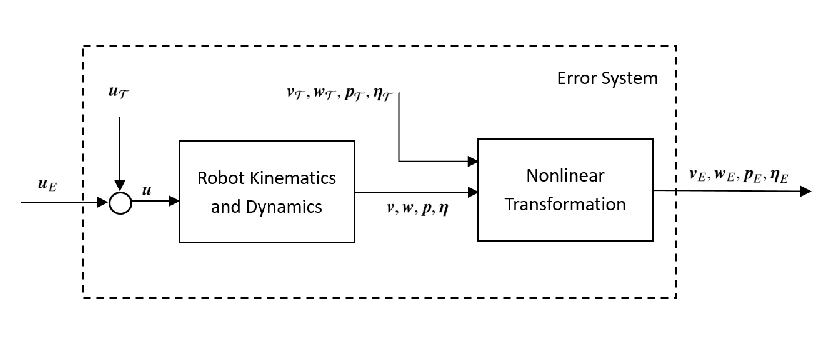
\includegraphics[width=3in]{errordynamics.eps}
\caption{Error System}
\label{ErrorSystem}
\end{figure}
Suppose the robot should track $m$ trim trajectories, which can be combined as \emph{motion primitives} to form a complex path. By implementing the aforementioned nonlinear transformation and linearizing at the trim equilibrium points, we will obtain $m$ linearized error dynamic systems 
\begin{equation}
 	\dot{\vec{x}}_{E,j}=A_{E,j}\vec{x}_{E,1}+B_{E,j}\vec{u}_{E,j}, \quad \text{for} \,\, j=1, \cdots, m, j
 \end{equation} 
 representing the index for the trim trajectory, where $\vec{x}_{E,j}=(\vec{v}_{E,j}~\vec{w}_{E,j}~\vec{p}_{E,j}~\vec{\eta}_{E,j})^{T}$, the error dynamics system matrix
\begin{equation}
A_{E,j}=
\begin{bmatrix}
A_{d,j}^{d}&A_{k,j}^{d}\\
I_{6 \times 6}&A_{d,j}^{d}
\end{bmatrix} \in \mathbb{R}^{12 \times 12}
\end{equation}
and the error dynamics input matrix 
\begin{equation}
B_{E,j}=
\begin{bmatrix}
B_{\vec{v},j} \\
B_{\vec{w},j} 
\end{bmatrix} \in \mathbb{R}^{12 \times (n_{t}+n_{f})}.
\end{equation}
For the complete trim path, we can formulate the error system along the $m$ trim trajectories as a switched system
\begin{align}
\Sigma_{S,A_{E},B_{E}}: \dot{\vec{x}}_{E}(t)=
A_{E}(t)\vec{x}_{E}(t)+B_{E}(t)\vec{u}_{E}(t),
\end{align}
where $A_{E}(t)\in\lbrace A_{E,1}, \cdots, A_{E,m}\rbrace$ and $B_{E}(t)\in\lbrace B_{E,1}, \cdots, B_{E,m}\rbrace$.
\subsection{Switched \ac{lqr}}
For each linearized trim segment, we design a \acl{lqr}  with weighting matrix $ \mathcal{Q}_{E,j}$ and $\mathcal{R}_{E,j}$, for $j=1, \cdots, m$, to minimize the cost function for the $j$-th trim trajectory
\begin{align}
J=\int^{\infty}_{0}[\vec{x}_{E,j}^{T}\mathcal{Q}_{E,j}\vec{x}_{E,j}+\vec{u}_{E,j}^{T}\mathcal{R}_{E,j}
\vec{u}_{E,j}]dt
\end{align}
subject to $\vec{x}_{E,j}(0)=\vec{x}_{E,j,0}$, $\mathcal{Q}_{E,j} \succeq 0$, $\mathcal{Q}_{E,j}^{T}=\mathcal{Q}_{E,j}$, $\mathcal{R}_{E,j} \succ 0$ and $\mathcal{R}_{E,j}^{T}=\mathcal{R}_{E,j}$.
Assuming that ($A_{E,j}$,~$B_{E,j}$) is controllable, the optimal solution to minimize the cost function is $\vec{u}_{E,j}=-\mathcal{K}_{j}\vec{x}_{E,j}$,
where $\mathcal{K}_{j}=\mathcal{R}_{E,j}^{-1}B_{E,j}^{T}
S_{E,j}$ is a constant linear state feedbak gain. The matrix $S_{E}\succeq 0$  which is the solution of the continuous \ac{are}: 
\begin{equation}
\mathcal{Q}_{E,j}+A_{E,j}^{T}S_{E,j}
+S_{E,j}A_{E,j}
-S_{E,j}B_{E,j}\mathcal{R}_{E,j}^{-1}
B_{E,j}^{T}S_{E,j}=0.
\end{equation}
The input vector of the actuators is $\vec{u}_{j}=\vec{u}_{E,j}+\vec{u}_{\mathcal{T}_{j}}
=\vec{u}_{\mathcal{T}_{j}}-\mathcal{K}\vec{x}_{E,j}$.  
When we implement the corresponding \ac{lqr} state feedback controllers to all trim trajectory segments, we obtain $\dot{\vec{x}}_{E,m} =(A_{E,j}-
\mathcal{R}_{E,j}B^{T}_{E,j}
\mathcal{S}_{E,j})\vec{x}_{E,j}$.
If we denote the closed-loop system matrix as $
\bar{A}_{E,j}=A_{E,j}-
\mathcal{R}_{E,j}B^{T}_{E,j}
\mathcal{S}_{E,j}$, we can represent the closed-loop error dynamics as a switched system
\begin{equation}
\Sigma_{S,\bar{A}_{E}}:\dot{\vec{x}}_{E}=\bar{A}_{E}(t)\vec{x}_{E},
\end{equation}
where $\bar{A}_{E}(t)\in\lbrace \bar{A}_{E,1}, \bar{A}_{E,2}, \ldots,\bar{A}_{E,m}\rbrace$.
An \ac{lqr} can ensure the stability of each trim trajectory segment, however it can not ensure the stability of the whole trajectory. The stability for arbitrary switching can be proven by means of \acfp{cqlf}, see~\cite{c7}. 

Recall that 
\begin{equation}
	V_{E,j}(\vec{x}_{E,j})=\vec{x}_{E,j}^{T}\mathcal{P}_{E,j}\vec{x}_{E,j}
\end{equation} is a \ac{qlf} for the \ac{lti} system 
\begin{equation}
	\vec{x}_{E,j}=\bar{A}_{E,j}(t)\vec{x}_{E,j}(t),
\end{equation} where $\mathcal{P}_{E,j}$ is symmetric and positive definite satisfying $\mathcal{P}_{E,j}\bar{A}_{E,j}
+\bar{A}_{E,j}^{T}\mathcal{P}_{E,j}$ being negative definite. The existence of \ac{cqlf} $V(\vec{x}_{E})=\vec{x}_{E}^{T}\mathcal{P}_{E}\vec{x}_{E}$ is equivalent to determine whether such a matrix $\mathcal{P}_{E}$ exists for a given group of Hurwitz matrices $\left\lbrace \bar{A}_{E,1}, \bar{A}_{E,2}, \ldots,\bar{A}_{E,m}\right\rbrace$ such that 
\begin{equation}
	\bar{A}_{E,m}^{T}\mathcal{P}_{E}
+\mathcal{P}_{E}\bar{A}_{E,m}  \prec 0.
\end{equation}
This is a system of \ac{lmi}, which is said to be feasible if a solution $\mathcal{P}_{E}$ exists. Otherwise, the LMIs are infeasible. 
Thus, determining whether or not the switched system $\Sigma_{S,\bar{\emph{\textbf{A}}}_{E}}$ has a CQLF amounts to checking the feasibility of a system of \ac{lmi}. 
We can convert these to the nonstrict \ac{lmi} 
$
\bar{A}_{E,m}^{T}\mathcal{P}_{E}
+\mathcal{P}_{E}\bar{A}_{E,m}  \preceq I
$ and 
$
\mathcal{P}_{E} \succeq I
$.
This can be formulated as semidefinite programming, which can be solved for example with the CVX toolbox by~\cite{c12,c13}, to check whether a matrix $\mathcal{P}_{E}$ satisfying the aforementioned \ac{lmi} can be found. 

%!TEX root=../root.tex

%%%%%%%%%%%%%%%%%%%%%%%%%%%%%%%%%%%%%%%%%%%%%%%%%%%%%%%%%%%%%%%%%%%%%%%%%%%%%%%%
%2345678901234567890123456789012345678901234567890123456789012345678901234567890
%        1         2         3         4         5         6         7        
\section{NUMERICAL SIMULATION}
In order to verify the proposed switched \ac{lqr} for the modular model, we apply rapid prototyping in MATLAB/SIMULINK. The robot geometric configuration parameters are adapted from the \emph{Snookie} robot configuration described in~\cite{c9}, which serves as a baseline. The robot possesses four horizontal thrusters, two vertical thrusters, two horizontal fins and two vertical fins as actuators, see Fig~\ref{snookie}. The thrust force is constrained to a range of $[-35\textup{N},40\textup{N}]$ , and the deflection angle is constrained within $[-20^\circ,20^\circ]$. The desired trim paths consist of seven segments whose parameters are specified in Table~\ref{TABLE:TrimSpecifications}. The robot should track the seven trajectories in $150$ seconds. Note that the yaw rate $\dot{\phi}_{\mathcal{T}}$ can not be set to zero due to the singularity problem of (\ref{EQ:pT}). Instead, we use a very small value ($10^{-6}$) to tackle this problem. From the specifications and geometric configuration parameters, we can derive the linearized error systems for each trim trajectory segment: $A_{E,1}, \cdots, A_{E,7}$ and $B_{E,1}, \cdots, B_{E,7}$. The initial state error $\vec{x}_{E,1}$ is set to be $\vec{0}$. The drag coefficient $c_{D}$ and lift coefficient $c_{L}$ are set to be equal $0.1$ and $0.001$, respectively. 

\begin{figure}[htb]
	\begin{center}
		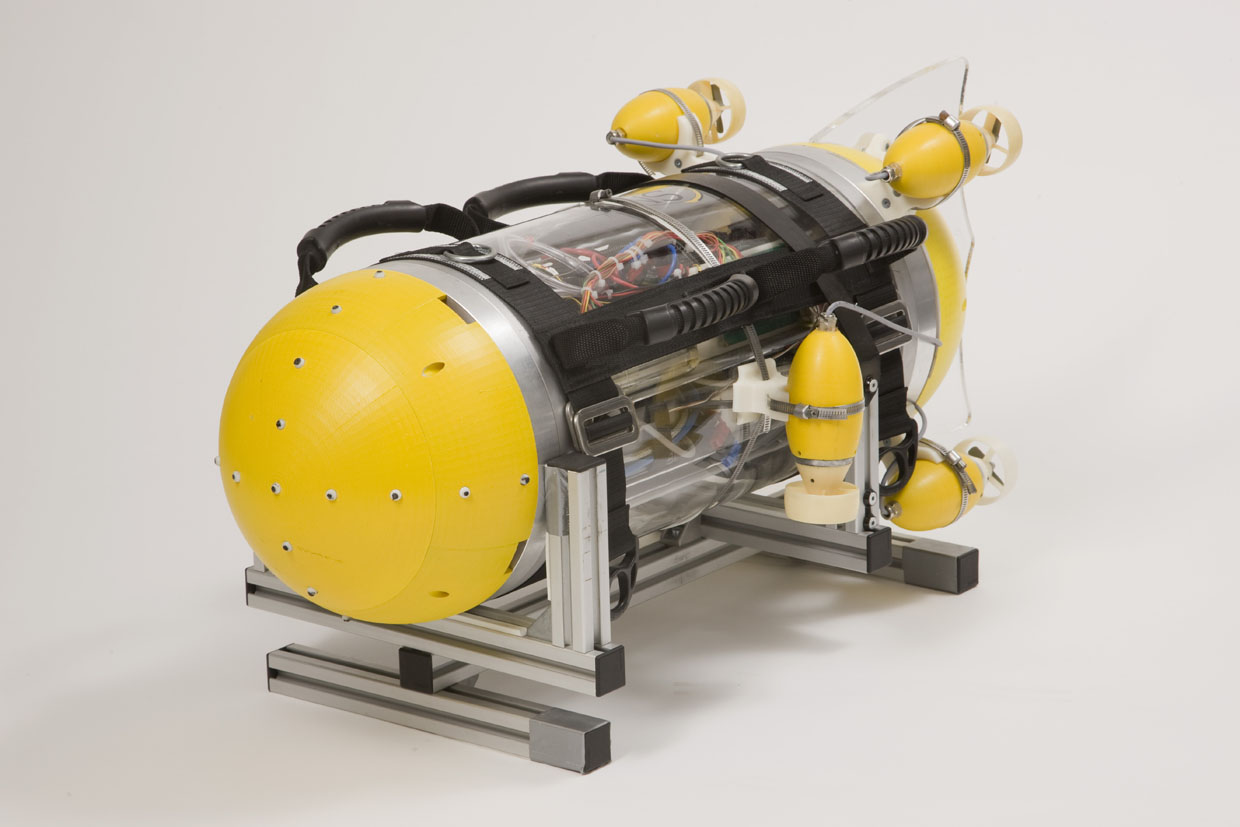
\includegraphics[width=.3\textwidth]{figures/Cotesys_Snookie_150dpi}
		\caption{\emph{Snookie} \ac{auv}}
		\label{snookie}
	\end{center}
\end{figure}
   
\begin{table}[htb]
\caption{Trim trajectories specifications}
\label{TABLE:TrimSpecifications}
\begin{center}
\begin{tabular}{| c | c | c | c | c |}
\hline
Segment&Time(s)&$||\vec{v}_{\mathcal{T}}||$ (m/s)&$\dot{\psi}_{\mathcal{T}}$ (rad/s)&$\gamma_{\mathcal{T}}$ (rad)\\ \hline
1&0-20&0.5&0&0\\ %\hline
2&20-30&0.5&0.0803&0 \\ %\hline
3&30-40&0.5&0.0803&0.2 \\ %\hline
4&40-50&0.5&0&0.2 \\ %\hline
5&50-60&0.5&-0.0803&0.2 \\ %\hline
6&60-70&0.5&-0.0803&0 \\ %\hline
7&70-150&0.5&0&0 \\ \hline
\end{tabular}
\end{center}
\end{table}  
 The state cost matrices for the individual trim segments are: 
\begin{align*}
	\mathcal{Q}_{1/2/4/5}&=diag([10^3, 10^3, 10^3, 300, 300, 300, 1, 1, 1, 1, 1, 1])\\
	\mathcal{Q}_{3}&=diag([10^3, 10^3, 10^3, 1, 1, 1, 1, 1, 1, 1, 1, 1])\\
	\mathcal{Q}_{6/7}&=diag([10^3, 10^3, 10^3, 10^3,  10^3, 10^3, 1, 1, 1, 1, 1, 1]),
\end{align*}
 The input weighting matrices are:
\begin{align*}
	\mathcal{R}_{2/3/4/5}&=diag([10^{-4},~\ldots~,10^{-4}, 10^{-3}, 10^{-3}, 10^{-3}, 10^{-3}])\\
	\mathcal{R}_{1/6}&=diag([10^{-4},~\ldots~,10^{-4}]) ~ \in \mathbb{R}^{12 \times 10}\\
	\mathcal{R}_{7}&=diag([10^{-5},~\ldots~,10^{-5}, 10^{-4}, 10^{-4}, 10^{-4}, 10^{-4}])
\end{align*}
Using these values, we can design an \ac{lqr} for each linearized error system and obtain state feed back gains $\mathcal{K}_{1}, \cdots, \mathcal{K}_{7}$.

In order to ensure the global stability of the formulated switched system under implementation of the \ac{lqr} with the selected weighting matrices, we check the existence of the common symmetric matrix $\mathcal{P}_{E}$ by solving the following optimization problem: 
\begin{equation}
	\min_{\mathcal{P}_{E}\in \mathbb{R}^{12 \times 12}}\mathrm{tr}(\mathcal{P}_{E}),
\end{equation} 
subject to $\bar{A}_{E,j}^{T}\mathcal{P}_{E}+\mathcal{P}_{E}\bar{A}_{E,j} \preceq I_{12 \times 12}$, $\mathcal{P}_{E} \succeq I_{12 \times 12}$, where $\bar{A}_{E,j}=A_{E,j}-\mathcal{K}_{j}$, $j=1, \cdots, 7$. Using the semidefinite programming in CVX~(\cite{c12,c13}), we could obtain the optimization result. For the current values of state cost matrices and input cost matrices, the objective function $\mathrm{tr}(\mathcal{P}_{E})$ has a feasible solution of $1891.49$, such that the corresponding positive definite symmetric matrix $\mathcal{P}_{E}$ can be used to prove the global stability of the linear switched error system. 

The reference trim trajectories and the tracked path of the underwater robot during the simulation are illustrated in Fig.~\ref{FIG:TrackingResult} and the corresponding error states $\vec{p}_{E}, \vec{\eta}_{E}, \vec{v}_{E}, \vec{w}_{E}$ are shown in Fig~\ref{FIG:ErrorStates}. If there is no actuator constraint, the robot can realize perfect tracking with the switched \ac{lqr}. For practical implementation, the control inputs are constrained by the capabilities of the actuators, as illustrated in Fig.~\ref{FIG:ControlInputs}. For tracking the first and the second trim segment along which the flight angle equals zero, the robot can nearly realize perfect tracking. When it moves downwards with flight angle $0.2$ rad, all error states rise and oscillate obviously, especially the pitch error $\vec{\theta}_{E}$. Another increase of state errors happens at the moment when the flight path angle $\gamma_{T}$ falls from $0.2$ to $0$. The changing of flight angle results in huge error and strong oscillations of the pitch error. At $70$ seconds, the yaw rate becomes zero suddenly, with a large roll velocity error $\vec{p}_{E}$ appearing consequently. Although we implement an \ac{lqr} for each trim trajectory segment, the controller can not drive the error states to zero before switching to the next trim segment. The remaining errors are the initial values for the next error dynamic system. In order to show the convergence performance of the error states under the implemented \ac{lqr}, we extend the duration of the last trim segment to $80$ seconds. From Fig.~\ref{FIG:ErrorStates}, we can see that the error states converge gradually to zero. 

\begin{figure}[htb]
\centering
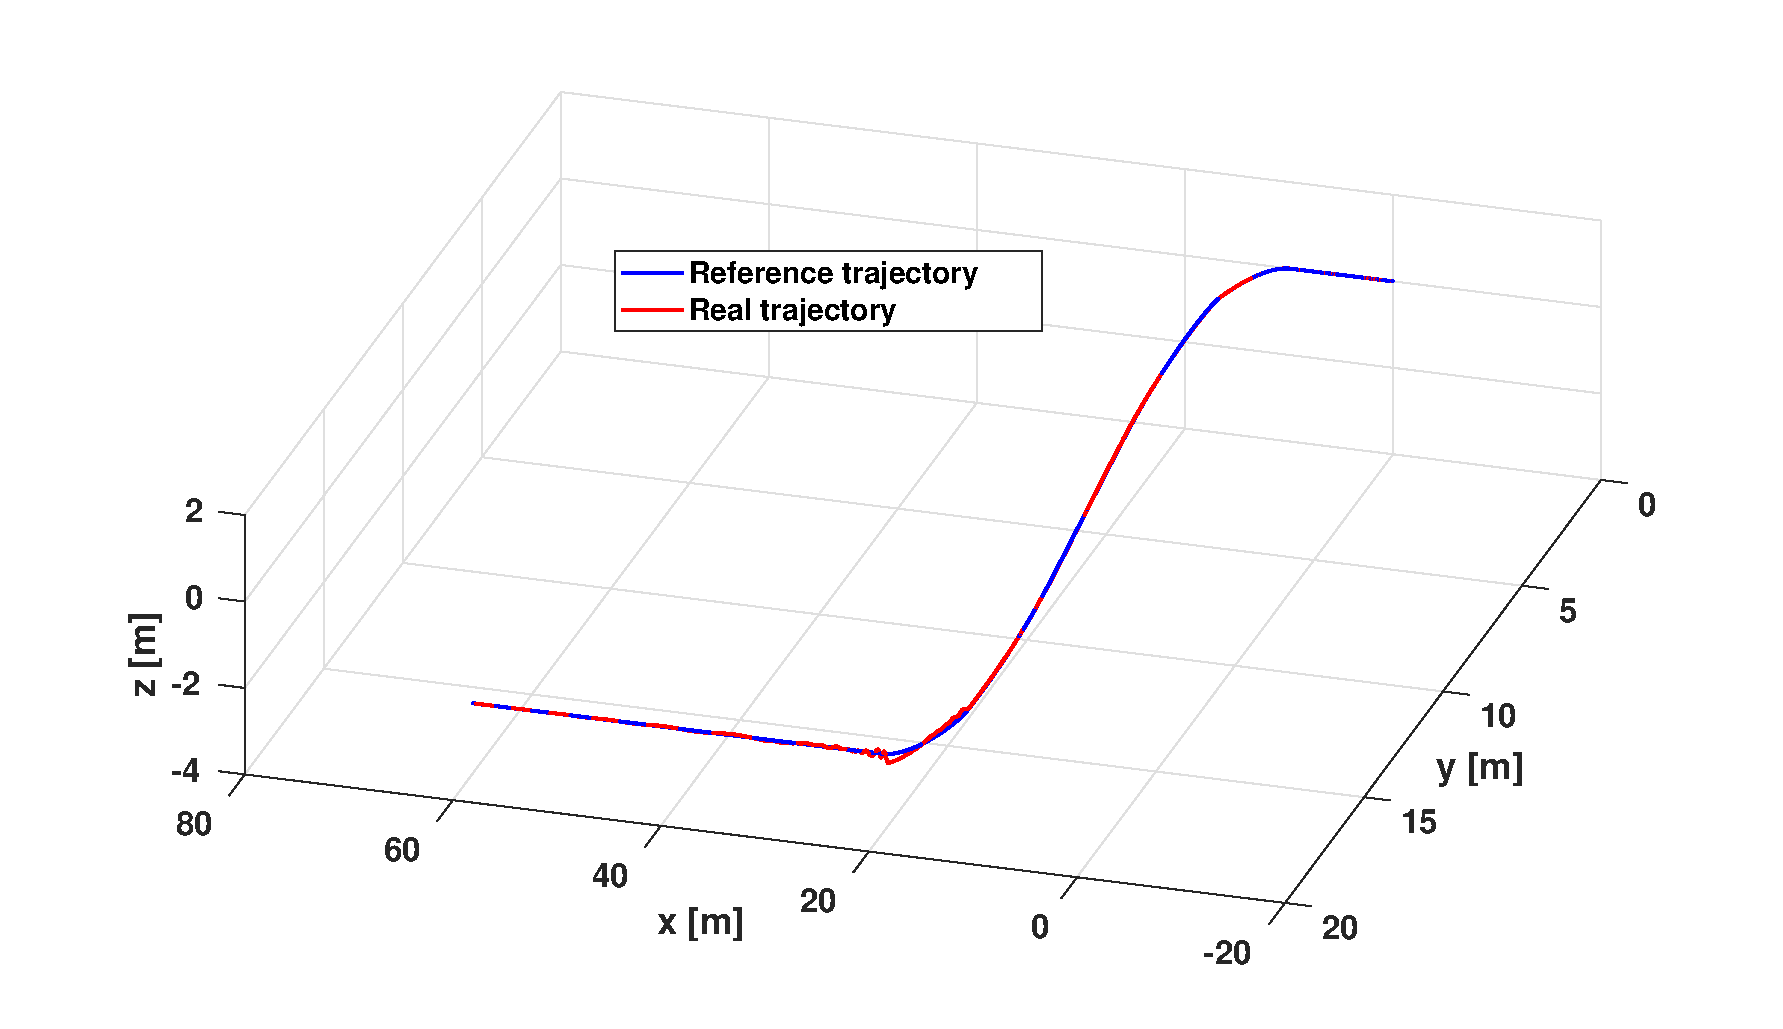
\includegraphics[width=3.5in]{TrajTracking.eps}
\caption{Tracking result}
\label{FIG:TrackingResult}
\end{figure}
\begin{figure}[htb]
\centering
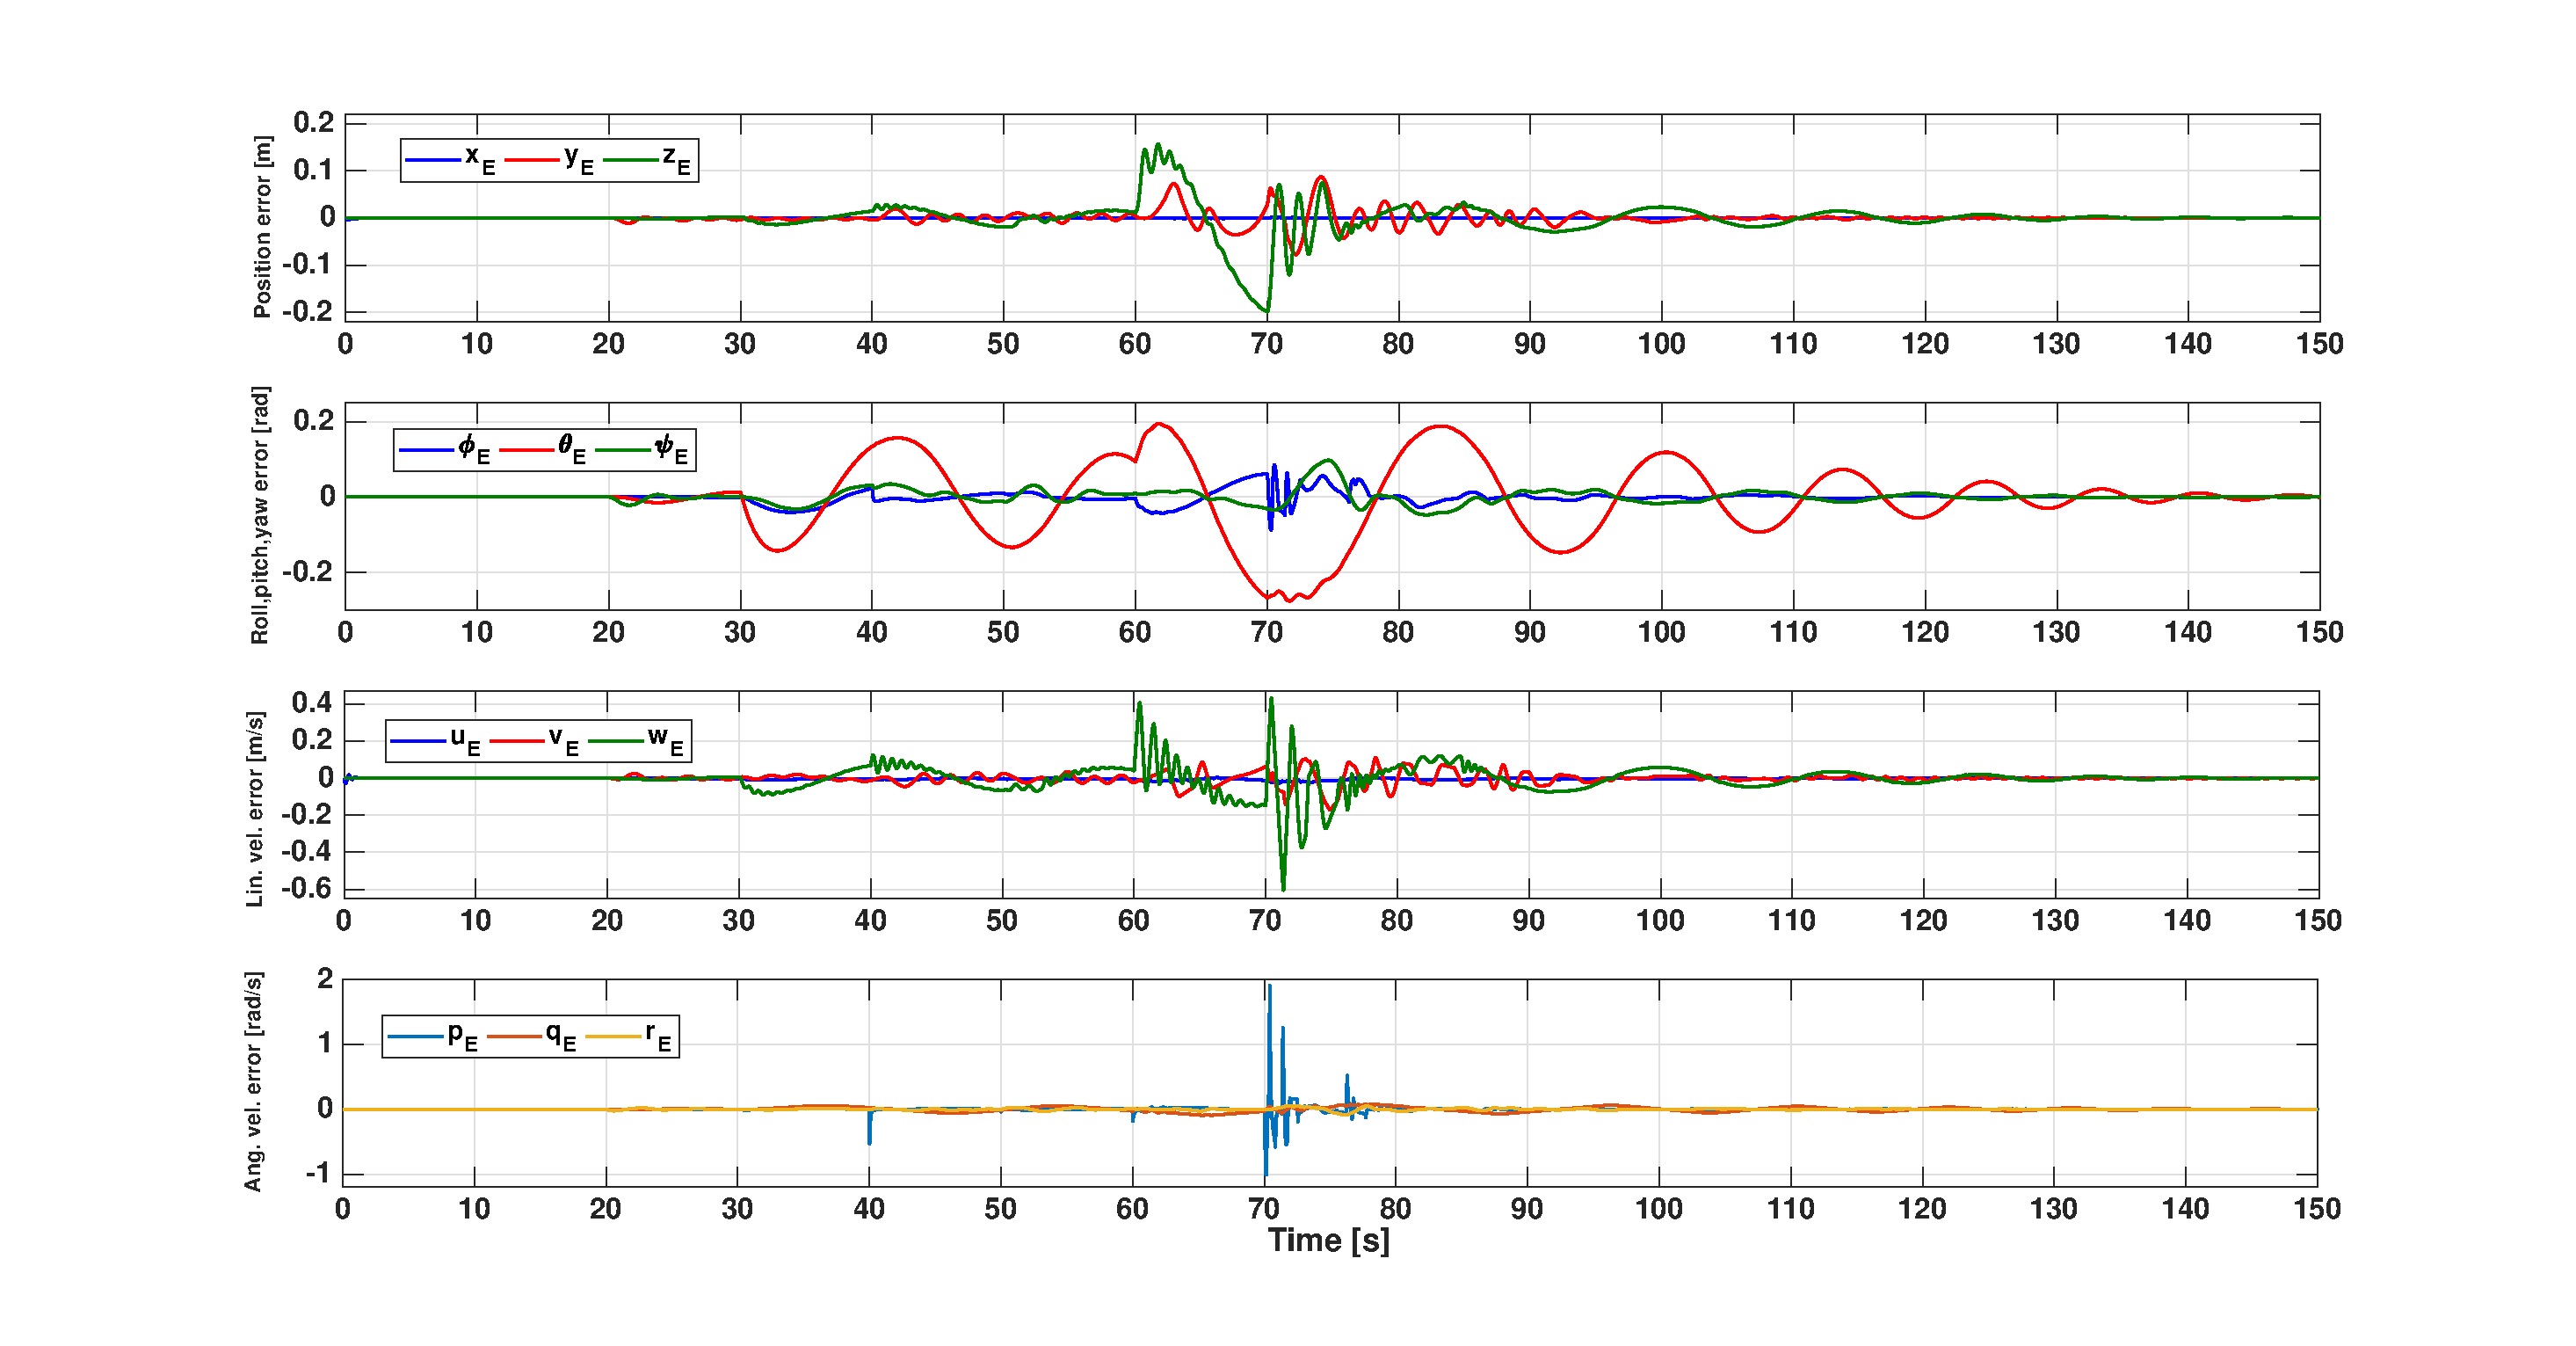
\includegraphics[width=3.5in]{StateError.eps}
\caption{Error states}
\label{FIG:ErrorStates}
\end{figure}

\begin{figure}[thpb]
\centering
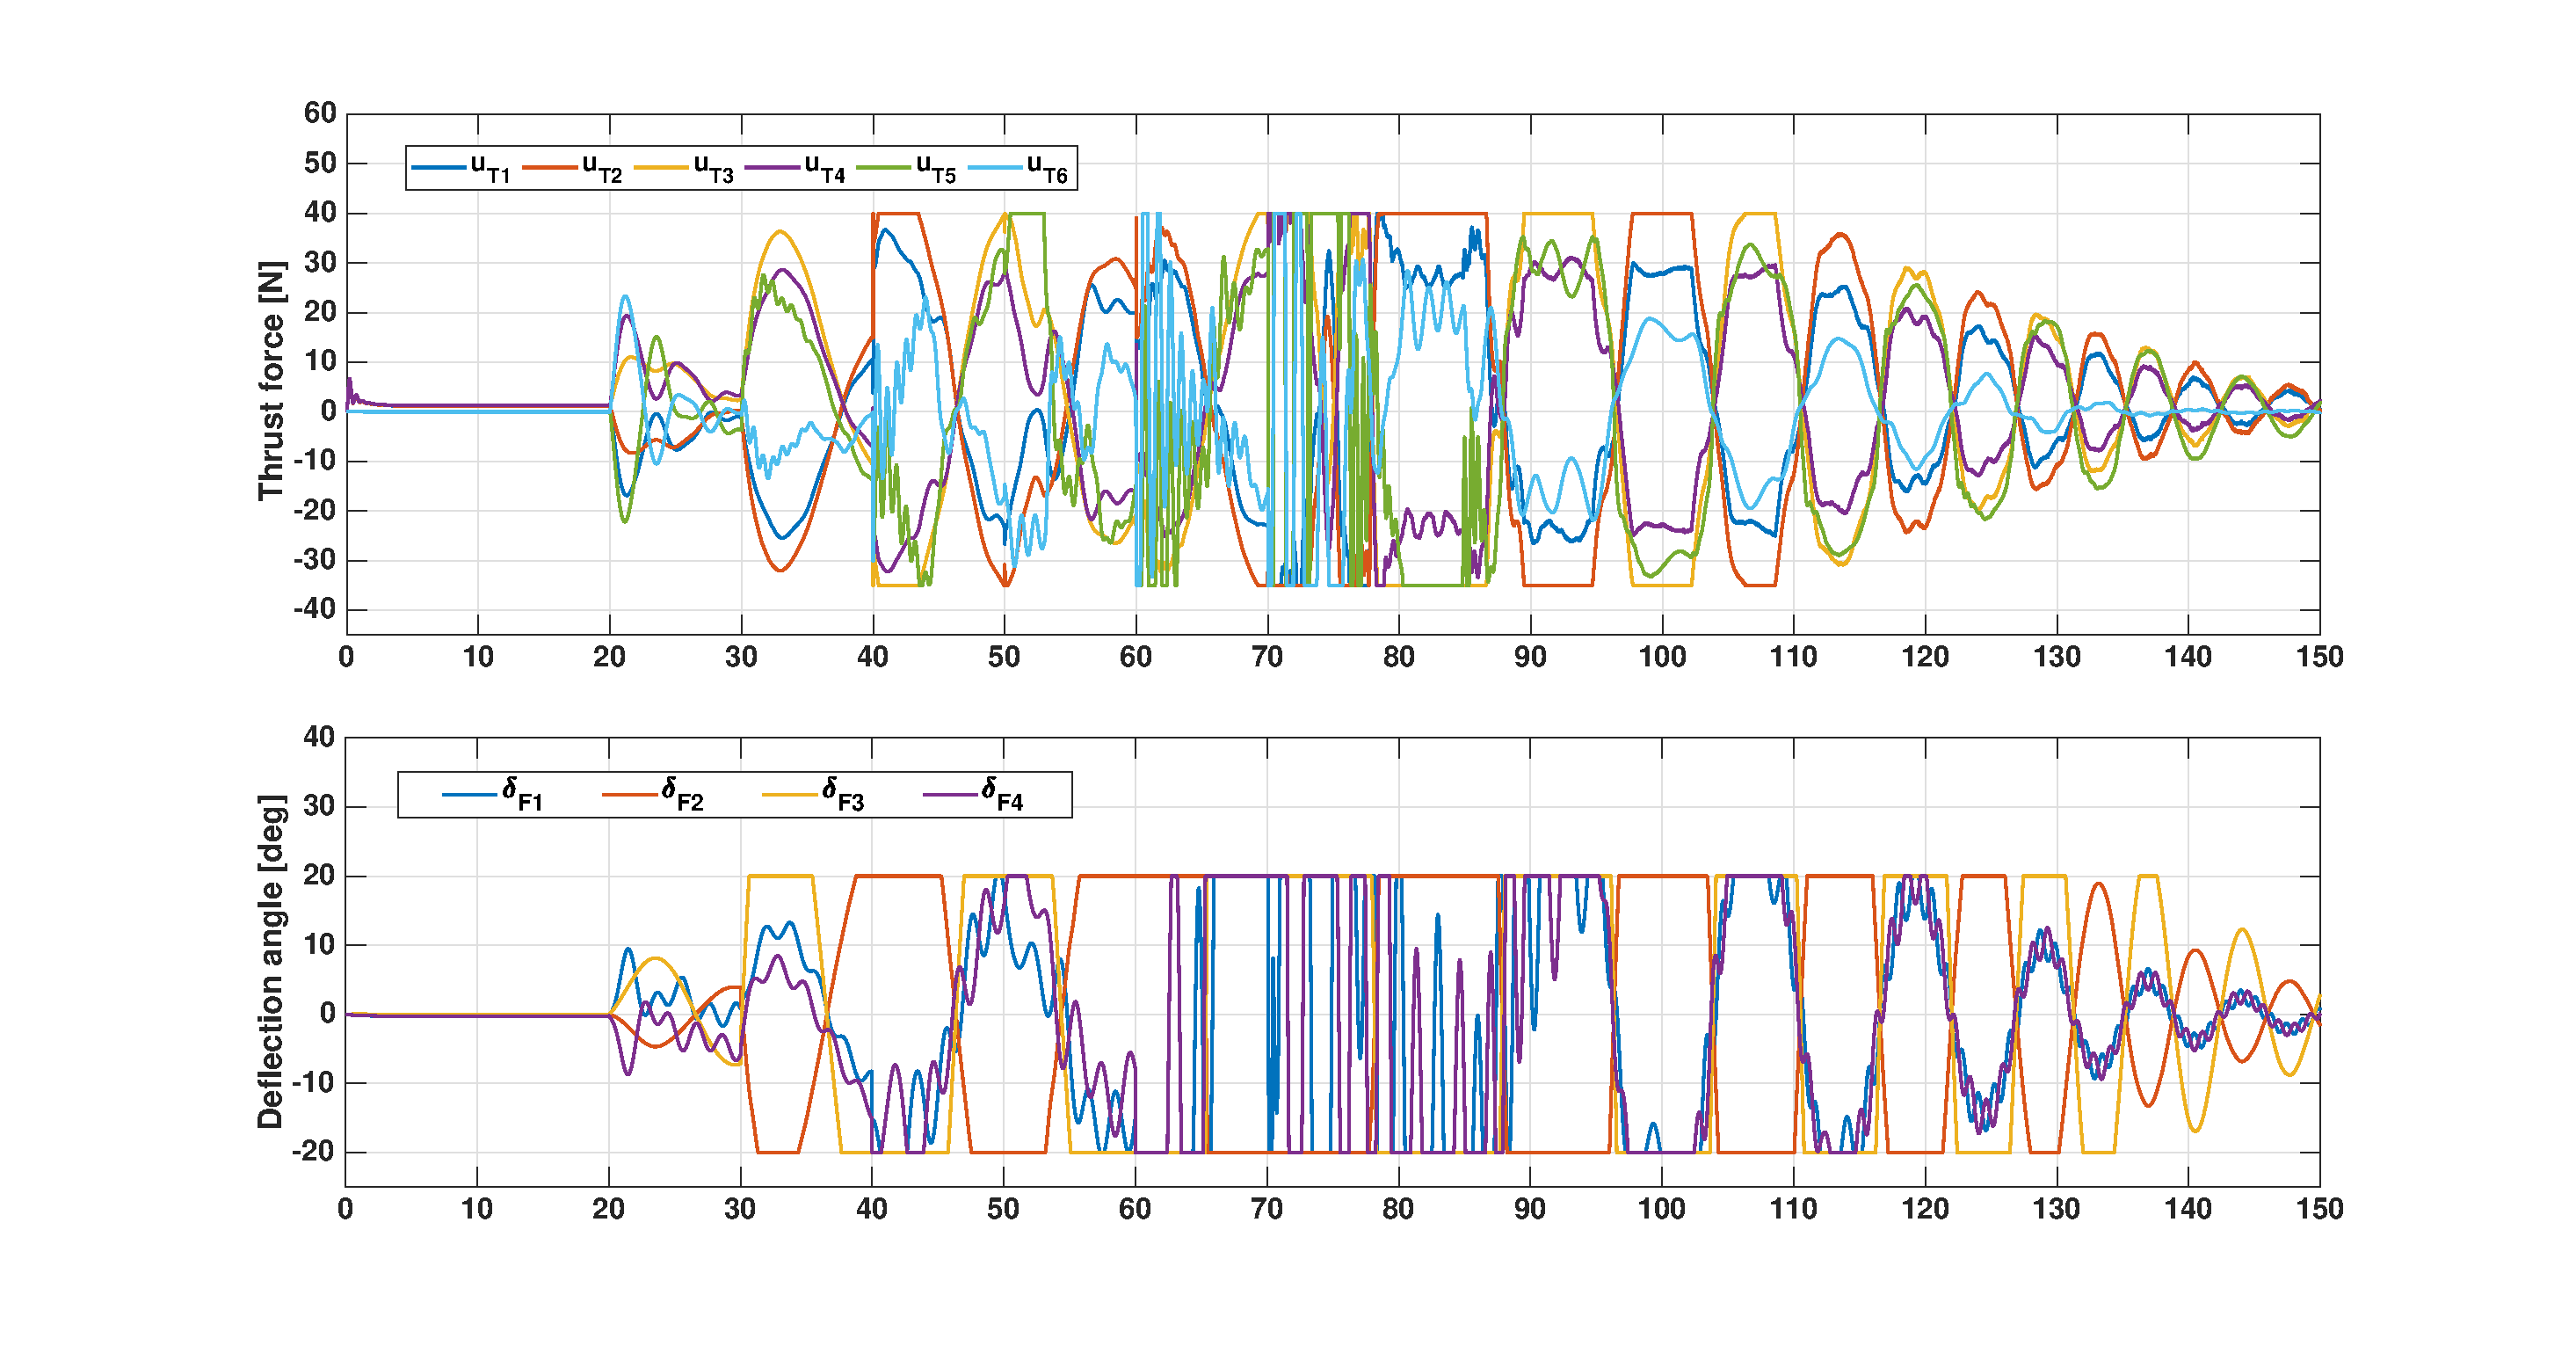
\includegraphics[width=3.5in]{InputPlot.eps}
\caption{Thrust force and deflection angle}
\label{FIG:ControlInputs}
\end{figure}

In summary, each trim path switching leads to a deviation of the real trajectory from the desired one. A switched \ac{lqr} control strategy with suitably chosen state and input weighting matrices can ensure the global stability and drive the robot to track the reference trajectory.


%!TEX root=../root.tex

%%%%%%%%%%%%%%%%%%%%%%%%%%%%%%%%%%%%%%%%%%%%%%%%%%%%%%%%%%%%%%%%%%%%%%%%%%%%%%%%
%2345678901234567890123456789012345678901234567890123456789012345678901234567890
%        1         2         3         4         5         6         7        
\newpage
\section{CONCLUSIONS}
In preparation for formulating the geometric design procedure as an optimization algorithm, in this paper we introduce a new modular modeling approach for (autonomous) underwater vehicles. The focus is on the identification of the geometric decision variables and their couplings both for the overall kinematic and kinetic design of the robot as well as the control allocation. In addition, we propose a method to formulate the robot dynamics as a linear \ac{mimo} switched system based on the task-determined trim trajectories and synthesize subsequently a switched \ac{lqr} controller, which can be checked for global stability. This enables a novel fully automatic task-dependent co-design of an \ac{auv} and its controller. The simulation results demonstrate that, in the unconstrained actuator case, the proposed model and control strategy can be successfully applied to perfectly track a set of predefined trim trajectories. However, the results also show that since \ac{lqr} does not explicitly consider actuator constraints, the tracking performance under more realistic conditions are suboptimal. To take the actuator constraints into consideration, a switched Model Predictive Controller (MPC) or a Linear parameter-varying (LPV) control approach is suggested for future work. 
%%%%%%%%%%%%%%%%%%%%%%%%%%%%%%%%%%%%%%%%%%%%%%%%%%%%%%%%%%%%%%%%%%%%%%%%%%%%%%%%
% \addtolength{\textheight}{-12cm}   % This command serves to balance the column lengths
                                  % on the last page of the document manually. It shortens
                                  % the textheight of the last page by a suitable amount.
                                  % This command does not take effect until the next page
                                  % so it should come on the page before the last. Make
                                  % sure that you do not shorten the textheight too much.

%%%%%%%%%%%%%%%%%%%%%%%%%%%%%%%%%%%%%%%%%%%%%%%%%%%%%%%%%%%%%%%%%%%%%%%%%%%%%%%%



%%%%%%%%%%%%%%%%%%%%%%%%%%%%%%%%%%%%%%%%%%%%%%%%%%%%%%%%%%%%%%%%%%%%%%%%%%%%%%%%



%%%%%%%%%%%%%%%%%%%%%%%%%%%%%%%%%%%%%%%%%%%%%%%%%%%%%%%%%%%%%%%%%%%%%%%%%%%%%%%%
% \section*{APPENDIX}

% Appendixes should appear before the acknowledgment.

% \section*{ACKNOWLEDGMENT}

% The preferred spelling of the word �acknowledgment� in America is without an �e� after the �g�. Avoid the stilted expression, �One of us (R. B. G.) thanks . . .�  Instead, try �R. B. G. thanks�. Put sponsor acknowledgments in the unnumbered footnote on the first page.



%%%%%%%%%%%%%%%%%%%%%%%%%%%%%%%%%%%%%%%%%%%%%%%%%%%%%%%%%%%%%%%%%%%%%%%%%%%%%%%%

% References are important to the reader; therefore, each citation must be complete and correct. If at all possible, references should be commonly available publications.



\begin{thebibliography}{99}
\bibitem[Antonelli(2003)]{c10} Antonelli, G., Underwater Robots. Berlin Heidelberg: Springer, 2003.
\bibitem[Bestaoui et~al.(2007)]{c3} Bestaoui, Y. and Hima, S., Modelling and trajectory generation of lighter-than-air aerial robots-invited paper, in Robot Motion and Control 2007, 3-28. London: Springer, 2007.
\bibitem[Chen(2007)]{c15} Chen, Y., Modular modeling and control for autonomous underwater vehicle (auv). Master�s thesis, National University of Singapore, Dept. of Mechanical Engineering, 2007.
\bibitem[Cunha et~al.(2005)]{c6} Cunha, R. and Silvestre, C., A 3D Path-Following Velocity-Tracking Controller for Autonomous Vehicles, in 16th IFAC World Congress, Praha, Czech Republic, 2005, July.
\bibitem[Du et~al.(2016)]{c1} Du, T., Schulz, A., Zhu, B., Bickel, B., and Matusik, W.. Computational multicopter design. ACM Trans. Graph., 35(6):227:1-227:10, November 2016.
\bibitem[Grant et~al.(2008)]{c12} Grant, M. and Boyd, S., Graph implementations for nonsmooth convex programs. In V. Blondel, S. Boyd, and H. Kimura, editors, Recent Advances in Learning and Control, Lecture Notes in Control and Information Sciences, pages 95-110.  Springer-Verlag Limited, 2008. 
\bibitem[Grant et~al.(2014)]{c13} Grant, M. and Boyd, S., CVX: Matlab software for disciplined convex programming, version 2.1. {http://cvxr.com/cvx}, March 2014.
\bibitem[Kaminer et~al.(1998)]{c5} Kaminer, I. and Pascoal, A. and Hallberg, E. and Silvestre, C., Trajectory Tracking for Autonomous Vehicles: An Integrated Approach to Guidance and Control, AIAA Journal of Guidance, Control, and Dynamics, 21(1): 29-38, 1998.
\bibitem[Nahon(1996)]{c14} Nahon, M., A simplified dynamics model for autonomous underwater vehicles, Proceedings of Symposium on Autonomous Underwater Vehicle Technology, Monterey, CA, 1996, pp. 373-379. doi: 10.1109/AUV.1996.532437
\bibitem[Sebbane(2014)]{c2} Sebbane, Y. B., Planning and Decision Making for Aerial Robots. Berlin Heidelberg: Springer, 2014.
\bibitem[Shorten et~al.(2007)]{c7} Shorten, R., Wirth, F., Mason, O., Wulff, K., and King, C., Stability Criteria for Switched and Hybrid Systems. SIAM Review, 49(4):545-592, 2007.
\bibitem[Shuzhe et~al.(2011)]{c16} Shuzhe, C., Soon, H. G., Hong, E. Y. and Chitre, M., Modular modeling of autonomous underwater vehicle, OCEANS'11 MTS/IEEE KONA, Waikoloa, HI, 2011, pp. 1-6. doi: 10.23919/OCEANS.2011.6106921
\bibitem[Silvestre et~al.(2002)]{c4} Silvestre, C., Pascoal, A., and Kaminer, I., On the design of gain-scheduled trajectory tracking controllers. International Journal of Robust and Nonlinear Control, 12(9):797-839, 2002.
\bibitem[Tang(1999)]{c11} Tang, S., Modeling and simulation of the autonomous underwater vehicle, autolycus. Master's thesis, Massachusetts Institute of Technology, Dept. of Ocean Engineering, 1999.
\bibitem[Vollmayr et~al.(2014)]{c9} Vollmayr, A.N., Sosnowski, S., Hirche, S., and van Hemmen, J.L., Snookie:
an autonomous underwater vehicle with artificial lateral line system. In Horst Bleckmann, Joachim Mogdans, and Sheryl L. Coombs, editors, Flow Sensing in Air and Water, chapter 20, pages 521-562. Springer Berlin Heidelberg, Berlin, Heidelberg, viii edition, 2014.
\bibitem[Yoerger et~al.(1990)]{c8} Yoerger, v,  Cooke, J. G., and  Slotine, J. J. E., The influence of thruster
dynamics on underwater vehicle behavior and their incorporation into control system design. IEEE Journal of Oceanic Engineering, 15(3):167-178, July 1990.
\end{thebibliography}
\end{document}
